
\documentclass[12pt,twoside,openany]{book}

%%% define a macro \ifpdf para compilação condicional -- PDF ou
%%% DVI/PS.
\usepackage{tikz}

\usepackage[ruled]{algorithm2e}
\renewcommand{\listalgorithmcfname}{Lista de Algoritmos}%
\renewcommand{\algorithmcfname}{Algoritmo}%

%\usepackage{subfigure}
\usepackage{subfloat}
%\usepackage{wrapfigure}
%%% acentuação
%\usepackage[latin1]{inputenc}
%\usepackage[brazil]{babel}

\usepackage[brazilian]{babel}
\usepackage[utf8]{inputenc}
\usepackage[T1]{fontenc}

%%% bibliografia
%\usepackage{chicago}
%\usepackage{natbib}
%\usepackage[square,sort,comma,numbers]{natbib}
\usepackage{latexsym}
\usepackage{breakcites}

\usepackage{setspace}
%\usepackage{mathptm}
\usepackage{latexsym}
\usepackage{amssymb}
\usepackage{xspace}
\usepackage{colortbl}

\usepackage{acronym}
%%% referencias com página \vref
\usepackage[brazil]{varioref}

%%% identa primeiro parágrafo
\usepackage{indentfirst}

%%% figuras um ao lado do outro
\usepackage{subfig}


%%% definir títulos de seção
\usepackage[sf,sl,outermarks]{titlesec}


%%% para tabelas
\usepackage{multirow}

%%% boxes
\usepackage{fancybox}
\usepackage{fancyvrb}
\usepackage{color}

%%% somente na versão PDF

%%% Para inclusão de gráficos
%\usepackage[pdftex]{graphicx}
\usepackage{graphicx}

%%% dimensões do documento
\usepackage{geometry}
  \geometry{a4paper,left=3cm,right=3cm,top=2.0cm,bottom=2cm,twoside}

%%% cria links no arquivo .pdf
%%% comentar as linhas na versão para impressao
\usepackage[pdfpagelabels,pagebackref]{hyperref}
%\usepackage{hyperref}


%%% propriedades do arquivo .pdf
\hypersetup{
    pdftitle = {},
    pdfsubject = {},
    pdfkeywords = {},
    pdfauthor = {}
    }




\hypersetup{colorlinks=true,linkcolor=black,citecolor=black,hypertexnames=false}

%%fonte
\usepackage{bookman}
\usepackage[T1]{fontenc}

%%para os numeros reais
\usepackage{amsfonts}
\usepackage{amsmath}

\DeclareFixedFont{\numberfont}{T1}{phv}{bx}{n}{2cm}

%%% redefine o formato do título



\titleformat{\chapter}[display]
  {\normalfont\Large\sffamily
  }
  {%\titlerule[3pt]%
   \filright
   \rule[32pt]{.7\linewidth}{4pt}
   \hspace{-11pt}
   \shadowbox{
   \begin{minipage}{.18\linewidth}
     \begin{center}
       \textsc{\Large\chaptertitlename}\\
       \vspace{1ex}
       {\numberfont\color[gray]{0.5} \thechapter}\\
       \vspace{1ex}
     \end{center}
   \end{minipage}}
  }
  {0pt}
  {\filcenter
   \Huge
   }
  [\hfill\rule{.8\textwidth}{0.5pt}\\
     \vskip-1.8ex\hfill\rule{.7\textwidth}{3pt}]


%%% macro para destacar a(s) primeira(s) letra do texto
%%% é necessário ter a fonte courier instalada
%
%  um texto do tipo:
%
%  \begin{document}
%    \versal{IN} THE beginning God created the heaven and the earth.  Now the
%    earth was unformed and void, and darkness was upon the face of the
%    deep; and the spirit of God hovered over the face of the waters.
%  \end{document}
%
%  irá produzir algo como:
%
%  I I\  I THE beginning God  created the heaven and  the earth.
%  I I \ I Now the earth was unformed and void, and darkness was
%  I I  \I upon the face of the deep; and the spirit of God hov-
%  ered over the face of the waters.

%\font\largefont= pzcmi scaled 6500

\newcommand{\versal}[1]{{\noindent
    \setbox0\hbox{\largefont #1 }%
    \count0=\ht0                   % height of versal
    \count1=\baselineskip          % baselineskip
    \divide\count0 by \count1      % versal height/baselineskip
    \dimen1 = \count0\baselineskip % distance to drop versal
    \advance\count0 by 1\relax     % no of indented lines
    \dimen0=\wd0                   % width of versal
    \global\hangindent\dimen0      % set indentation distance
    \global\hangafter-\count0      % set no of indented lines
    \hskip-\dimen0\setbox0\hbox to\dimen0{\raise-\dimen1\box0\hss}%
    \dp0=0in\ht0=0in\box0}}
% Backref com colocação de "Citado na página..."
\renewcommand*{\backref}[1]{}
\renewcommand*{\backrefalt}[4]{
   \ifcase #1
       Não citado no texto.
   \or
       Citado na página~#2.
   \else
       Citado nas páginas #2.
   \fi
}

\renewcommand{\backreftwosep}{ e~}
\renewcommand{\backreflastsep}{, e~}


\usepackage{pgf}
\usepackage{baseboxes}
\usepackage{basecolor}

\newcommand{\natr}{{n_{at}}}
\newcommand{\nexe}{{n_{ex}}}
\newcommand{\ncls}{{n_{cl}}}
\newcommand{\nseg}{{n_{sg}}}
\newcommand{\di}{{D_1}}
\newcommand{\dii}{{D_2}}



\newcommand{\palestra}{\textit{palestra}\xspace}
\newcommand{\relevancia}{\hbox{\textit{relevância}}}
\newcommand{\distancia}{\hbox{\textit{distância}}}
\newcommand{\comida}{\hbox{\textit{comida}}}
\newcommand{\brinde}{\hbox{\textit{brinde}}}

\newcommand{\rankeadores}{\textit{rankeadores}\xspace}
\newcommand{\rankeador}{\textit{rankeador}\xspace}
\newcommand{\rankings}{\textit{rankings}\xspace}
\newcommand{\ranking}{\textit{ranking}\xspace}
\newcommand{\classificadorScore}{classificador \textit{score}\xspace} 
\newcommand{\classificadoresScore}{classificadores \textit{score}\xspace}
\newcommand{\estimadorProbabilidade}{\textit{estimador de probabilidade}\xspace} 
\newcommand{\estimadoresProbabilidade}{\textit{estimadores de probabilidade}\xspace} 
\newcommand{\segmento}{\textit{segmento}\xspace}
\newcommand{\segmentos}{\textit{segmentos}\xspace}
\newcommand{\adjacente}{\textit{adjacente}\xspace}
\newcommand{\adjacentes}{\textit{adjacentes}\xspace}
\newcommand{\grosseiro}{\textit{grosseiro}\xspace}
\newcommand{\refinado}{\textit{refinado}\xspace}

\newcommand{\overfitting}{\textit{overfitting}\xspace}


\newcommand{\jfe}{\textit{J48}\xspace}
\newcommand{\cfourfive}{\textsc{C4.5}\xspace}
\newcommand{\lexrank}{\textsc{LexRank}\xspace}
\newcommand{\lexprob}{\textsc{LexProb}\xspace}
\newcommand{\calinb}{\textsc{CaliNB}\xspace}

\newcommand{\progroc}{\textsc{ProgROC}\xspace}
\newcommand{\cotraining}{\textsc{Co-training}\xspace}
\newcommand{\corai}{\textsc{Corai}\xspace}
\newcommand{\nb}{\textsc{naive Bayes}\xspace}
\newcommand{\ie}{\textit{i.e.}\xspace}

\newcommand{\mc}{\hbox{\textit{c}}}
\newcommand{\mvp}{\hbox{\textit{VP}}}
\newcommand{\mfp}{\hbox{\textit{FP}}}
\newcommand{\mfn}{\hbox{\textit{FN}}}
\newcommand{\mvn}{\hbox{\textit{VN}}}

\newcommand{\mpos}{\hbox{\textit{Pos}}}
\newcommand{\mneg}{\hbox{\textit{Neg}}}

\newcommand{\mppos}{\hbox{\textit{PPos}}}
\newcommand{\mpneg}{\hbox{\textit{PNeg}}}

\newcommand{\mtotal}{\hbox{\textit{Total}}}

\newcommand{\mtvp}{\hbox{\textit{TVP}}}
\newcommand{\mtfp}{\hbox{\textit{TFP}}}

\newcommand{\tvp}{\textit{TVP}\xspace}
\newcommand{\tfp}{\textit{TFP}\xspace}

\newcommand{\vp}{\textit{VP}\xspace}
\newcommand{\fp}{\textit{FP}\xspace}
\newcommand{\fn}{\textit{FN}\xspace}
\newcommand{\vn}{\textit{VN}\xspace}


\newcommand{\ipos}{\textit{Pos}\xspace}
\newcommand{\ineg}{\textit{Neg}\xspace}


\newcommand{\total}{\textit{Total}\xspace}

\newcommand{\score}{\textit{score}\xspace}
\newcommand{\scores}{\textit{scores}\xspace}
\newcommand{\stm}{\textit{steamming}\xspace}

\newcommand{\stems}{\textit{stems}\xspace}
\newcommand{\stem}{\textit{stem}\xspace}

\newcommand{\precisao}{\textit{precisão}\xspace}
\newcommand{\oddsratio}{\textit{odds ratio}\xspace}
\newcommand{\posteriorodds}{\textit{posterior odds}\xspace}



\newtheorem{theorem}{Teorema}[chapter]
\newtheorem{corollary}[theorem]{Corolário}
\newtheorem{definition}{Definição}[chapter]
\newtheorem{example}{Exemplo}[chapter]


\newcommand{\chat}{\mbox{$\hat{c}$}}
\newcommand{\rhat}{\mbox{$\hat{r}$}}
\newcommand{\shat}{\mbox{$\hat{s}$}}
\newcommand{\phat}{\mbox{$\hat{P}$}}
\newcommand{\mhat}{\mbox{$\hat{m}$}}
\newcommand{\ghat}{\mbox{$\hat{g}$}}
\newcommand{\x}{\mbox{\textbf{x}}}
\newcommand{\nkp}{n_k^+}
\newcommand{\nkn}{n_k^-}

\newcommand{\adviolator}{\textit{adjacent violator}\xspace}
\newcommand{\adviolators}{\textit{adjacent violators}\xspace}

\newcommand{\gram}{gram\xspace}
\newcommand{\grams}{\textit{grams}\xspace}
\newcommand{\cbr}{\textsc{cbr}\xspace}
\newcommand{\ilp}{\textsc{ilp}\xspace}



\newcommand{\pretext}{\textsc{PreTexT}\xspace}
\newcommand{\news}{{\sc news}\xspace}
\newcommand{\course}{{\sc course}\xspace}
\newcommand{\lnai}{{\sc lnai}\xspace}
\newcommand{\ccourse}{{\tt course}\xspace}
\newcommand{\cncourse}{{\tt non-course}\xspace}
\newcommand{\sci}{{\tt sci}\xspace}
\newcommand{\talk}{{\tt talk}\xspace}
\newcommand{\texto}{\textsc{text}\xspace}
\newcommand{\links}{\textsc{links}\xspace}


\newcommand{\nni}{\textsc{9nni}\xspace}
\newcommand{\mode}{\textsc{mode}\xspace}


\newcommand{\brierScore}{\textit{Brier score}\xspace}



\begin{document}

\pagestyle{empty}
\pagenumbering{roman}

%%% insere a capa
%%% edite os campos para título, data, orientador e nome

\newcommand{\titulo}{Contador de objetos em vídeos usando redes neurais convolucionais}
  

\begin{titlepage}


\ \vfill

\begin{center}
\begin{minipage}[c]{12cm}
\begin{center}
\hrulefill\\
\vspace{.5cm} {\Large \titulo}\\
\vspace{1.3cm}
\textbf{\it Plabiany Rodrigo Acosta}\\
\vspace{.5cm}
\hrulefill\\
\end{center}
\end{minipage}
\end{center}

\vfill

\cleardoublepage


\begin{flushright}
\begin{Sbox}
\begin{minipage}{8.5cm}
\footnotesize
SERVIÇO DE  PÓS-GRADUAÇÃO FACOM - UFMS\\
\\
Data de Depósito: \\
\\
Assinatura:\hrulefill
\end{minipage}
\end{Sbox}
\fbox{\TheSbox}
\end{flushright}


\vspace*{2cm}
\begin{center}
{\huge\sf \titulo}\footnote{FACOM-UFMS}


\vspace*{2cm}

{\it Plabiany Rodrigo Acosta}

\vspace*{2cm}


{\bf Orientador:}  {\it Profº Drº Wesley Nunes Gonçalves}

\end{center}

\vspace*{4cm}

\begin{flushright}
\begin{minipage}{10cm}
Dissertação de Mestrado apresentada a Faculdade de Computação - FACOM - UFMS como parte dos requisitos necessários à obtenção do título de Mestre em Ciências de Computação.
\end{minipage}
\end{flushright}

\vspace*{2cm}
\begin{center}
\textbf{MS - Campo Grande \\março/2021}
\end{center}
\cleardoublepage



\end{titlepage}

%\cleardoublepage

\pagestyle{plain}


\onehalfspacing

\ \\
\vspace{80ex}

\begin{flushright}
\it
  Aos meus pais,\\
  Plácido Acosta e Eusebia P. Villalva,\\

\vspace{3ex}

  Aos meus irmãos,\\
  Vanessa Cristina Acosta e Luiz César V. Acosta,\\

\vspace{3ex}
  Aos meus sobrinhos,\\
  Luiz Carlos A. Acosta e Larissa A. Acosta.
\end{flushright}



\cleardoublepage
\chapter*{Agradecimentos}

		A Deus que reside em mim e que se faz presente em minha respiração no dia-a-dia.
		
		Aos meus pais Plácido Acosta e Eusebia Parede Villalva Acosta, a minha irmã Vanessa Cristina Acosta e ao meu irmão Luiz Cézar Villalva Acosta, por todo o apoio e amor que já recebi e ainda vou receber deles.

		Ao Prof. Dr. Wesley Nunes Gonçalves por conduzir e ter idéias que tornaram este trabalho realidade.
		A Universidade Federal de Mato Grosso do Sul (UFMS).
		

%  Nem sempre a resposta está pronta. Há uma beleza na dúvida que vale à pena de
%  ser apreciada. Forjar a resposta antes do tempo é a mesma coisa que colher
%  frutos verdes.



%\cleardoublepage
\chapter*{Abstract}
%English Text

This work presents a method of Neural Network Convolutional (CNN) to count and locate objects in videos through density maps.
Each object is represented by a dot only. In this way a 2D Gaussian core is applied at each point to originate the \textit{Ground Truth} of the density map.
The method receives a frame from the video in an instant $t$ and the frame in the instant $ t-1 $. In this way, the time displacement vectors of the objects are estimated, and a refinement of the density map takes place through stages.

A comparison of the number of stages used in the refinement branches is presented, as well as a variation of $\sigma$ to generate the \textit{Ground Truth} of the objects.

% stages (E) were also used to refine the predicted confidence map.
The proposed method was evaluated by the FISHCV155V database, developed by the UCDB INOVISÃO group in partnership with IFMS and Projeto Pacu. In this context, the count of fingerlings, which are newly hatched fish and move thoughtlessly, was analyzed and tested. The architecture obtained $MAE = 0.11$ and $\textit{F-measure} = 98\%$ with $\sigma = 1.1$, using the time displacement vector of the objects. The method demonstrated that the vector of displacement of the objects can assist in the detection and the labeling in the point type can be the way to count excessive amounts of objects in an image.



\chapter*{Resumo}

Este trabalho apresenta um método de Rede Neural Convolutional (CNN) para contar e localizar objetos em vídeos através de mapas de densidade. 
Cada objeto é representado por um ponto apenas. Desta forma um núcleo Gaussiano 2D é aplicado em cada ponto para originar o \textit{Ground Truth} do mapa de densidade.
O método recebe um quadro do vídeo em um instante $t$ e o quadro no instante $t-1$. Desta forma Vetores de Deslocamento Temporal dos objetos são estimados, e um refinamento do mapa de densidade acontece através de estágios. 
São apresentados um comparativo na quantidade de estágios utilizados nos ramos de refinamento, e uma  variação de $\sigma$ para geração do \textit{Ground Truth} dos objetos.

%estágios (E) também foram utilizados para refinar o mapa de confiança previsto. 
O método proposto foi avaliado pelo banco de dados FISHCV155V, desenvolvido pelo grupo INOVISÃO da UCDB em parceria com o IFMS e a empresa Projeto Pacu. Neste contexto foi analisado e testado a contagem de alevinos, que são peixes recém chocados e se movem irrefletidamente. A arquitetura obteve $MAE = 0.11$ e $\textit{F-measure} = 98\%$ com $\sigma = 1.1$, utilizando o vetor de deslocamento temporal dos objetos. O método demonstrou que o vetor de deslocamento dos objetos pode auxiliar na detecção e a rotulação no tipo ponto pode ser o caminho para contar quantidades excessivas de objetos em uma imagem.  

%Ao utilizar 2 quadros auxiliares, a técnica obteve erro médio absoluto (MAE) de 0.12, um erro quadrático médio de raiz (RMSE) igual a 0, coeficiente de determinação ($R^2$) igual a 0,977 e a média harmônica da métrica F1 igual a 98.4\% de acertos. O método demonstrou ser eficiente na localização e contagem de alevinos


%As 4 primeiras camadas da VGG19 foram aplicadas para estimar o mapa de recursos e camadas convolucionais foram empregadas para aprimorar tal mapa de maneira com que a presença do(s) alevino(s) nas imagens se sobressaia(m) ao fundo. O método utiliza a presciência das localizações dos peixes nos quadros anteriores para um refinamento do mapa de densidade do quadro atual. A arquitetura proposta foi ratificada através de experimentos com vídeos do mundo real. A média harmônica da métrica F1 obteve uma exatidão de 98,4\% na contagem utilizando como reforço o deslocamento realizado pelo alevino através da posição onde ele se encontrava no quadro anterior. A métrica de erro NRMSE obteve o valor 0, e as métricas MAE e MSE obtiveram valores 0.12 e 0.15 sucessivamente.

%Portuguese Text

%This paper presents a Convolutional Neural Network (CNN) approach for counting and locating ob-jects with high-ensity. To the best of our knowledge, this is the first object counting and locatingmethod based on a feature map enhancement and a Multi-tage Refinement of the confidence map.The proposed method was evaluated in two counting data-ets: tree and car. For the tree data-et, ourmethod returned a mean absolute error (MAE) of 2.05, a root-ean-quared error (RMSE) of 3.57and a coefficient of determination (R 2 ) of 0.977. In the car data-et (CARPK and PUCPR+), ourmethod was superior to state-f-he-rt methods like Deep-oU-NN, VGG-AP-R, VGG-AP,LPN, RetinaNet, and others. In the CARPK and PUCPR+ data-ets, it achieved an MAE of 4.45 and3.16, an RMSE of 6.18 and 4.39, and an R 2 of 0.975 and 0.999, respectively. The method is suitablefor dealing with high object-ensity, returning a state-f-he-rt performance for counting and locatingobjects.

%The purpose of this work is to develop computational intelligence models based on neuralnetworks (NN), fuzzy models (FM), support vector machines (SVM) and long short-erm memorynetworks (LSTM) to predict human pose and activity from image sequences, based on computervision approaches to gather the required features. To obtain the human pose semantics (outputclasses), based on a set of 3D points that describe the human body model (the input variablesof the predictive model), prediction models were obtained from the acquired data, for example,video images. In the same way, to predict the semantics of the atomic activities that compose anactivity, based again in the human body model extracted at each video frame, prediction modelswere learned using LSTM networks. In both cases the best learned models were implemented in anapplication to test the systems. The SVM model obtained 95.97\% of correct classification of the sixdifferent human poses tackled in this work, during tests in different situations from the training phase.The implemented LSTM learned model achieved an overall accuracy of 88\%, during tests in differentsituations from the training phase. These results demonstrate the validity of both approaches topredict human pose and activity from image sequences. Moreover, the system is capable of obtainingthe atomic activities and quantifying the time interval in which each activity takes place.
%\cleardoublepage
\tableofcontents
\addcontentsline{toc}{section}{Sumário}
\cleardoublepage

\listoffigures
\addcontentsline{toc}{section}{Lista de Figuras}
\cleardoublepage

\listoftables
\addcontentsline{toc}{section}{Lista de Tabelas}
\cleardoublepage


%\addcontentsline{toc}{section}{Lista de Abreviaturas}
%\cleardoublepage
%%\chapter*{Lista de Abreviaturas}
%\begin{acronym}
%  \acro{AD}[AD]{Árvore de Decisão}
%  \acro{AM}[AM]{Aprendizado de Máquina}
%  \acro{AUC}[AUC]{\textit{Area Under ROC Curve}}
%  \acro{EM}[EM]{{\em Expectation Maximization}}
%  \acro{FN}[FN]{Falso Negativo}
%  \acro{FP}[FP]{Falso Positivo}
%  \acro{IA}[IA]{Inteligência Artificial}
%  \acro{KDD}[KDD]{{\em Knowledge Discovery in Databases}}
%  \acro{LABIC}[LABIC]{Laboratório de Inteligência Computacional}
%  \acro{LR}[LR]{\textit{Likelihood Ratio}}
%  \acro{MAP}[MAP]{\textit{Maximum a Posteriori}}
%  \acro{MCAR}[MCAR]{\textit{Missing Completely at Random}}
%  \acro{MT}[MT]{Mineração de Texto}
%  \acro{NB}[NB]{\textit{Naive Bayes}}
%  \acro{OD}[OD]{\textit{Odds Ratio}}
%  \acro{PAV}[PAV]{\textit{Pool Adjacent Violators}}
%  \acro{PET}[PET]{\textit{Probability Estimation Trees}}
%  \acro{ROC}[ROC]{\textit{Receiver Operating Characteristic}}
%  \acro{SVM}[SVM]{{\em Support Vector Machines}}
%  \acro{TFP}[TFP]{Taxa de Falso Positivo}
%  \acro{TVP}[TVP]{Taxa de Verdadeiro Positivo}
%  \acro{VN}[VN]{Verdadeiro Negativo}
%  \acro{VP}[VP]{Verdadeiro Positivo}
%\end{acronym}


%\cleardoublepage


%\listofalgorithms
%\addcontentsline{toc}{section}{Lista de Algoritmos}
%\cleardoublepage




%%% inserir resumo
%\chapter*{Abstract}
%English Text

This work presents a method of Neural Network Convolutional (CNN) to count and locate objects in videos through density maps.
Each object is represented by a dot only. In this way a 2D Gaussian core is applied at each point to originate the \textit{Ground Truth} of the density map.
The method receives a frame from the video in an instant $t$ and the frame in the instant $ t-1 $. In this way, the time displacement vectors of the objects are estimated, and a refinement of the density map takes place through stages.

A comparison of the number of stages used in the refinement branches is presented, as well as a variation of $\sigma$ to generate the \textit{Ground Truth} of the objects.

% stages (E) were also used to refine the predicted confidence map.
The proposed method was evaluated by the FISHCV155V database, developed by the UCDB INOVISÃO group in partnership with IFMS and Projeto Pacu. In this context, the count of fingerlings, which are newly hatched fish and move thoughtlessly, was analyzed and tested. The architecture obtained $MAE = 0.11$ and $\textit{F-measure} = 98\%$ with $\sigma = 1.1$, using the time displacement vector of the objects. The method demonstrated that the vector of displacement of the objects can assist in the detection and the labeling in the point type can be the way to count excessive amounts of objects in an image.



\chapter*{Resumo}

Este trabalho apresenta um método de Rede Neural Convolutional (CNN) para contar e localizar objetos em vídeos através de mapas de densidade. 
Cada objeto é representado por um ponto apenas. Desta forma um núcleo Gaussiano 2D é aplicado em cada ponto para originar o \textit{Ground Truth} do mapa de densidade.
O método recebe um quadro do vídeo em um instante $t$ e o quadro no instante $t-1$. Desta forma Vetores de Deslocamento Temporal dos objetos são estimados, e um refinamento do mapa de densidade acontece através de estágios. 
São apresentados um comparativo na quantidade de estágios utilizados nos ramos de refinamento, e uma  variação de $\sigma$ para geração do \textit{Ground Truth} dos objetos.

%estágios (E) também foram utilizados para refinar o mapa de confiança previsto. 
O método proposto foi avaliado pelo banco de dados FISHCV155V, desenvolvido pelo grupo INOVISÃO da UCDB em parceria com o IFMS e a empresa Projeto Pacu. Neste contexto foi analisado e testado a contagem de alevinos, que são peixes recém chocados e se movem irrefletidamente. A arquitetura obteve $MAE = 0.11$ e $\textit{F-measure} = 98\%$ com $\sigma = 1.1$, utilizando o vetor de deslocamento temporal dos objetos. O método demonstrou que o vetor de deslocamento dos objetos pode auxiliar na detecção e a rotulação no tipo ponto pode ser o caminho para contar quantidades excessivas de objetos em uma imagem.  

%Ao utilizar 2 quadros auxiliares, a técnica obteve erro médio absoluto (MAE) de 0.12, um erro quadrático médio de raiz (RMSE) igual a 0, coeficiente de determinação ($R^2$) igual a 0,977 e a média harmônica da métrica F1 igual a 98.4\% de acertos. O método demonstrou ser eficiente na localização e contagem de alevinos


%As 4 primeiras camadas da VGG19 foram aplicadas para estimar o mapa de recursos e camadas convolucionais foram empregadas para aprimorar tal mapa de maneira com que a presença do(s) alevino(s) nas imagens se sobressaia(m) ao fundo. O método utiliza a presciência das localizações dos peixes nos quadros anteriores para um refinamento do mapa de densidade do quadro atual. A arquitetura proposta foi ratificada através de experimentos com vídeos do mundo real. A média harmônica da métrica F1 obteve uma exatidão de 98,4\% na contagem utilizando como reforço o deslocamento realizado pelo alevino através da posição onde ele se encontrava no quadro anterior. A métrica de erro NRMSE obteve o valor 0, e as métricas MAE e MSE obtiveram valores 0.12 e 0.15 sucessivamente.

%Portuguese Text

%This paper presents a Convolutional Neural Network (CNN) approach for counting and locating ob-jects with high-ensity. To the best of our knowledge, this is the first object counting and locatingmethod based on a feature map enhancement and a Multi-tage Refinement of the confidence map.The proposed method was evaluated in two counting data-ets: tree and car. For the tree data-et, ourmethod returned a mean absolute error (MAE) of 2.05, a root-ean-quared error (RMSE) of 3.57and a coefficient of determination (R 2 ) of 0.977. In the car data-et (CARPK and PUCPR+), ourmethod was superior to state-f-he-rt methods like Deep-oU-NN, VGG-AP-R, VGG-AP,LPN, RetinaNet, and others. In the CARPK and PUCPR+ data-ets, it achieved an MAE of 4.45 and3.16, an RMSE of 6.18 and 4.39, and an R 2 of 0.975 and 0.999, respectively. The method is suitablefor dealing with high object-ensity, returning a state-f-he-rt performance for counting and locatingobjects.

%The purpose of this work is to develop computational intelligence models based on neuralnetworks (NN), fuzzy models (FM), support vector machines (SVM) and long short-erm memorynetworks (LSTM) to predict human pose and activity from image sequences, based on computervision approaches to gather the required features. To obtain the human pose semantics (outputclasses), based on a set of 3D points that describe the human body model (the input variablesof the predictive model), prediction models were obtained from the acquired data, for example,video images. In the same way, to predict the semantics of the atomic activities that compose anactivity, based again in the human body model extracted at each video frame, prediction modelswere learned using LSTM networks. In both cases the best learned models were implemented in anapplication to test the systems. The SVM model obtained 95.97\% of correct classification of the sixdifferent human poses tackled in this work, during tests in different situations from the training phase.The implemented LSTM learned model achieved an overall accuracy of 88\%, during tests in differentsituations from the training phase. These results demonstrate the validity of both approaches topredict human pose and activity from image sequences. Moreover, the system is capable of obtainingthe atomic activities and quantifying the time interval in which each activity takes place.
%
%\newpage

%%% corpo do texto


\pagenumbering{arabic}

%%% inclua os seu arquivos a partir daqui


\chapter{Introdução}
 
 \section{Motivação e Lacuna}
 \label{sec:Motivacao}
%   A contagem de objetos deu origem aos números que suscetivamente originou os cálculos e conforme a evolução humana acontece técnicas para auxiliar a contagem e cálculos estão cada vez mais acentuada, pois em vários meios para se obter um resultado no mundo real, é necessário ainda mão de obra humana, além de requerer um certo tempo. 

%    A interação com humanoides faz parte do imaginário humano desde os períodos históricos. Através da capacidade computacional de processar dados, viu-se ali a possibilidade de tornar real a simulação da vida biológica em modelos matemáticos. A idealização da inteligência artificial estabeleceu a necessidade da Visão Computacional, área que abrange a habilidade de máquinas visualizarem e reconhecerem o contexto apresentado por imagens. Desde então Redes Neurais Artificiais tem sido aplicadas com o objetivo de detectar e predizer objetos, afim de compreender situações \cite{DBLP:journals/corr/BadrinarayananK15}. As subáreas como Aprendizagem de Máquina e Aprendizagem Profunda compreendem técnicas para detecção de certos padrões com a intenção de predizer itens presentes em figuras \cite{Goodfellow-et-al-2016}.
    
A aprendizagem profunda (\textit{Deep Learning}) tem se destacado no cenário de Visão Computacional e as Redes Neurais Convolucionais (CNN) \cite{Simonyan14c} tem dominado o estado da arte \cite{ANN}. Estudos podem ser encontrados para detecção de objetos \cite{DBLP:journals/corr/abs-1904-00889, 8437104, 8489369, rs11010011, 8186148}, segmentação de imagens \cite{Zhao2017CVPR,DBLP:journals/corr/CaoSWS16}, contagem de objetos \cite{8186148,DBLP:journals/corr/CaoSWS16,articleLuiz}, entre outros.
    
Entre as diversas aplicações da Visão Computacional, os métodos de contagem e localização de objetos consistem em detectar e obter a posição de cada objeto individualmente na imagem.
Esses métodos tem auxiliado no controle e contagem de pessoas \cite{ExtractHuman}, carros \cite{CarCount}, animais \cite{8639306}, e até mesmo bactérias \cite{7320116}.
    A maioria dos métodos de contagem são baseados nos mais conhecidos métodos de detecção de objetos (Faster-RCNN \cite{DBLP:journals/corr/Girshick15}, RetinaNet \cite{DBLP:journals/corr/abs-1708-02002}, YoloV3 \cite{DBLP:journals/corr/abs-1804-02767}).
    Esses métodos consideram um retângulo envolvente para cada objeto e podem fornecer tanto a posição (centro do retângulo envolvente) como a contagem (número de retângulos envolventes). 
    %Layout Proposal Networks (LPNs) \cite{8237708} é um método recente que tem seguido a proposta de detecção de objetos para contagem.
    
    Embora os métodos recentes tenham obtido resultados promissores, três desafios ainda se mantêm.
    O primeiro desafio é a alta densidade com objetos sobrepostos.
    Em geral, os métodos de detecção de objetos não são adequados para cenários densos de objetos \cite{Goldman2019CVPR}.
    Neste caso, a grande sobreposição dos retângulos envolventes devido a oclusão dificulta o aprendizado dos métodos. Layout Proposal Networks (LPNs) \cite{8237708} é um método recente que tem seguido a proposta de detecção de objetos para contagem de carros utilizando camadas da VGG-16. Seu maior problema na contagem está na sobreposição dos retângulos quando carros estão lado a lado na imagem, como em um estacionamento. 
    %Na vida real temos como preceito a idéia de que dois corpos não ocupam o mesmo espaço, as CNN's por sua vez detectam bordas, textura e cor de espaços pré-definidos nos experimentos (rotulação) através das camadas convolucionais nas imagens (\cite{deeplearningbook}).
    
    
    Por outro lado, estimar um mapa de densidade para obter a quantidade de objetos tem apresentado resultados promissores \cite{DBLP:journals/corr/abs-1808-01050,880968,Cao2017} e  feito com que estudos tenham esta direção.
    Um mapa de densidade consiste em estimar a probabilidade de um objeto ocorrer em cada pixel da imagem.
    Porém a diversidade encontrada nos cenários das imagens (e.g., escala, rotação, etc) dificulta a detecção e contagem por um mapa de densidade. Assim alguns trabalhos buscam encontrar um método eficaz que faça com que o objeto de interesse tenha um destaque nas probabilidades estimadas \cite{inproceedings} \cite{DBLP:journals/corr/abs-1711-04433}.
    
    O segundo desafio é a necessidade da rotulação detalhada das imagens, o que é difícil de obter em grandes quantidades. 
    A rotulação de um retângulo envolvente para cada objeto na imagem torna-se inviável para cenas muito densas em grandes quantidades de imagens.
     Por outro lado, a utilização de um único ponto para rotular cada objeto \cite{8237708} tem sido grande alvo de estudos.
     Por exemplo, \cite{DBLP:peri/corr/abs-1904-01333} propõem o método de detecção e contagem de multidões usando pontos na cabeça das pessoas. 
     Os métodos baseados apenas em pontos consideram a informação de contexto ao redor do ponto, pois os objetos compartilham cores, textura e forma.
     Dessa forma, os métodos tendem a reconhecer mesmo que os limites dos objetos não estejam delimitados durante o aprendizado \cite{Aich2018ImprovingOC}.

    O terceiro desafio consiste em contar e localizar objetos em uma sequência de imagens.
   A análise do movimento que objetos realizam nos vídeos podem fornecer informações valiosas que nem sempre são consideradas na contagem de objetos em uma imagem.
Nesse contexto, alguns pesquisadores demonstram em seus estudos que rastrear o movimento pode auxiliar na detecção e reconhecimento, assim como distingui-los do fundo (\cite{Ma_2015_ICCV,Nam_2016_CVPR,Danelljan_2015_ICCV_Workshops,WANG201962,8898173,ExtractHuman}).  
   Diferente do rastreamento de objetos, o objetivo deste trabalho é considerar as informações do passado para contar e localizar os objetos em um quadro atual.
    
    Para contornar os desafios citados acima, este trabalho propõe um método para localizar e contar objetos em vídeos usando redes neurais convolucionais.
    %Dada uma imagem de entrada
    Dado um quadro de um video e o quadro anterior, o método proposto estima uma mapa de densidade com a probabilidade de ocorrência de um objeto em cada pixel.
    Dessa forma, a rotulação apenas de pontos é suficiente para o treinamento do método e cenas densas podem ser melhor modeladas.
    %o método proposto considera as predições das posições dos objetos no quadro anterior.
    Além disso, o método proposto também estima um mapa de vetores de deslocamento, isto é, vetores que indicam a direção do movimento de cada pixel da imagem.
    Essa estimativa dos vetores de deslocamento também é usada para predizer o mapa de densidade de um quadro atual.
    Todas essa informações são concatenadas para estimar a localização e contagem de objetos do quadro atual.
    Resultados experimentais mostram que a concatenação dessas informações é capaz de melhorar a contagem e localização dos objetos.
    
    
    
    %Pontos estratégicos na posição de cada objeto é usado como rotulagem. A hipótese aposta nas posições por onde o objeto percorreu anteriormente para estimar o ponto onde ele pode ser encontrado.
    %O método é dividido em quatro fases principais: 1) geração do mapas de recurso usando a VGG19 para cada quadro processado; 2) refinamento do mapa de recursos usando as localizações anteriores; 3) estágios múltiplos de refinamento dos mapas de confiança combinados com o mapa obtido das posições anteriores; e 4) a obtenção da posição do objeto através de picos no mapa de confiança. Os parâmetros foram avaliados na contagem de alevinos presentes no conjunto de dados.


%    A contagem de peixes está entre um dos desafios a serem solucionados para se obter uma solução automática e rápida.
   
%   A pesca está presente no dia-a-dia de milhões de pessoas pelo mundo e pondera fortemente a alimentação, cultura e economia. Por ser o combustível de vários povos na história, se tornou fundamental na alimentação nos períodos modernos. Apesar de muitos grupos ainda utilizarem o peixe como fonte única de nutrição, a sua comercialização move uma porcentagem significativa da economia em vários países singulares na criação e exportação. A China, por exemplo, possui uma participação acima de 60\% da produção mundial de peixe \cite{OECD}\cite{FAO}.
   
%   A produção brasileira de peixes tem crescido nos últimos anos \cite{FAO}. Estima-se que o país latino-americano por possuir um clima favorável e recursos hídricos, possa ter um aumento de 104\% na produção pesqueira até o ano de 2025. Em 2018 a produção teve um crescimento de 4,5 toneladas\cite{EMBRAPA}. 

%   O estado de Mato Grosso do Sul-MS ocupa o 10º lugar na lista dos maiores produtores de peixes de cultivo do Brasil com 25.850 toneladas produzidas. O primeiro lugar vem sendo ocupado nos últimos anos pelo Paraná com 129.900 toneladas \cite{PeixeBR,OECD}.
   
%  O cultivo de peixes sofre grandes intervenções de mercado, com o objetivo de manter a segurança alimentar e ambiental \cite{Aqua}.
%  No sentido de corresponder a demanda mercantil, determinadas espécies necessitam de adaptações, para um clima específico e até mesmo alterações na alimentação.
%  Assim organizações de aquicultura (piscicultura) buscam opções tecnológicas para um máximo aproveito do produto comercializado.
  
%O foco principal desta dissertação está em 
  
  
  % produção de peixe continuará a aumentar para quase 200 Mt em 2026.

\section{Aplicação em Contagem de Peixes}
\label{sec:Aplicação}

%Aplicar técnicas de Aprendizado Profundo para automatizar a contagem de objetos presente em vídeos utilizando a análise do deslocamento de tais objetos no(s) quadro(s) anterior(es). Contudo, apresentar resultados que comprove tal hipótese utilizando vídeos do mundo real. Para realizar este feito os experimentos foram realizados com vídeos onde contém alevinos. 

O método proposto será aplicado na contagem de peixes e alevinos. Na maioria dos casos, a contagem é um trabalho árduo e requer mão de obra humana atenta, além de ser suscetível a erros.
Por serem sensíveis, os peixes requerem uma afabilidade no manuseio durante a contagem.
Em geral, a contagem acontece por técnicas de barragens \cite{Erikson}, alguns cultivadores realizam a peneiragem para extrair os peixes da água e, dessa maneira, obtêm-se uma estimativa da quantidade de peixes que residem em uma determinada região \cite{OECD,FAO}.


A escada de peixes é uma das maneiras utilizadas na contagem.
Assim os peixes passam por barragens conforme a Figura \ref{fig:escadadepeixes} (a). Na usina hidrelétrica de Igarapava do rio Grande \cite{UHE}, pesquisadores construíram salas (Figura \ref{fig:escadadepeixes} (b)) abaixo do nível d'água, sendo possível enxergar os peixes conforme eles atravessam.
Especialistas na área buscam encontrar técnicas para automatizar a contagem dos peixes que transitam a hidrelétrica.


\begin{figure}[!ht]
	\centering
		\subfloat[]{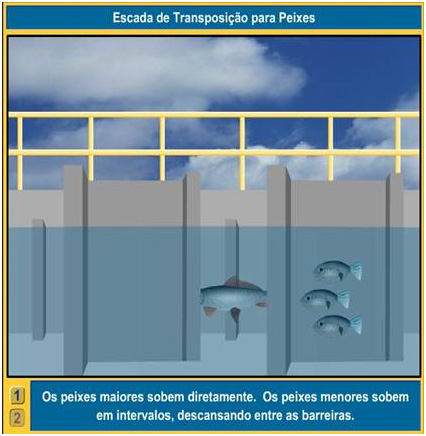
\includegraphics[width=0.4\textwidth]{image/escadadepeixes.jpg}}\vspace{0.3cm}
	    \subfloat[]{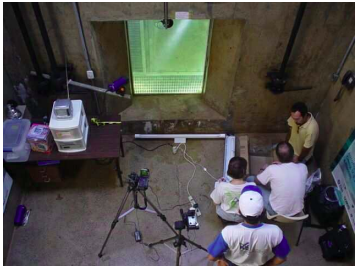
\includegraphics[width=0.55\textwidth]{image/saladaagua.png}}
	\caption{(a) Ilustração da Escada de peixes - \cite{UHE}, (b) sala abaixo do nível d'água \cite{Erikson}.}
	\label{fig:escadadepeixes}
\end{figure}

Os cultivadores precisam ter o controle da quantidade de peixes vivos presentes em seus cativeiros, para que a alimentação seja devidamente proporcional para todos, e se há necessidade do cultivo de novos peixes, ou até mesmo alterações no meio. É notória a necessidade de uma exatidão da quantidade que residem uma região. 


\section{Objetivos}
\label{sec:objetivos}

\section{Objetivo Geral}
O objetivo deste trabalho é propor um método para contagem de objetos em vídeos utilizando redes neurais convolucionais.
Um dos intentos principais está em detectar tais objetos nas imagens levando em consideração a posição espacial no quadro anterior. Assim com a ciência das localizações anteriormente, uma estimativa mais refinada da posição atual pode ser obtida.

%Os peixes presentes no \textit{dataset} utilizado se locomovem irrefletidamente e como foram recém chocados, possuem um tamanho muito reduzido quando comparado a fase adulta. Assim os alvos a serem alcançados está em analisar parâmetros que se adaptam a esses peixes de maneira que a contagem seja a mais exata possível.

\section{Objetivos Específicos}

%O foco dos experimentos pode ser descrito como uma análise dos parâmetros para aperfeiçoar a técnica proposta, de modo que se ajuste adequadamente ao conjunto de dados. 
%Os peixes presentes no \textit{dataset} utilizado se locomovem irrefletidamente e como foram recém chocados, possuem um tamanho muito reduzido quando comparado a fase adulta. Assim os alvos a serem alcançados está em analisar parâmetros que se adaptam a esses peixes de maneira que a contagem seja a mais exata possível.

Tendo o objetivo geral imposto, os seguintes objetivos específicos foram definidos:
%
\begin{enumerate}
    %\item Gerar um volume de entrada, contendo a imagem de entrada e os vetores de deslocamento dos objetos no quadro anterior.
    \item Estimar a contagem por meio de um mapa de densidade obtido por uma rede neural convolucional;
    \item Avaliar a inclusão do quadro anterior na estimativa do quadro atual;
    \item Incluir vetores de deslocamento na predição do mapa de densidade;
    \item Aplicar o método na contagem de alevinos.

\end{enumerate}

%Para alcançar os objetivos específicos foram realizadas as seguintes atividades:

%\begin{enumerate}
    %\item Rotular cada peixe presente nos quadros de maneira que os pontos represente cada alevino;
    %\item Gerar o \textit{Ground Truth} com base nos pontos para os quadros atuais e o um vetor de deslocamento para cada peixe;
    %\item Gerar o mapa de recursos para os quadros processados com a VGG19, depurar os mapas resultantes com estágios de refinamento.
    %\item Gerar o mapa de recursos do(s) quadro(s) anterior(es) dos quadros atuais processados com a VGG19, depurar os mapas resultantes com estágios de refinamento.
   % \item Concatenar os mapas dos quadros anteriores e atuais conforme os estágios são aplicados;
  %  \item Treinar a CNN proposta com vários parâmetros para o ajuste ao conjunto de dados;
 %   \item Estimar um linear para detectar os picos nos mapas de densidades resultantes do modelo treinado;
%    \item Testar e avaliar os resultados qualitativamente e quantitativamente;
%\end{enumerate}


%\section{Principais Contribuições}
%\label{sec:contribuicoes}


%\section{Organização}
%\label{sec:organizacao}



\chapter{Revis{\~{a}}o Bibliogr{\'{a}}fica}
\label{chap:am}

%\section{Fundamentação Teórica}

%Os computadores digitais modernos superam os humanos no domínio da computação numérica e manipulação de símbolos relacionados (\cite{ANN}). O surgimento de novas técnologias, novas capacidades computacionais facilita os estudos matemáticos que tem sido cada vez mais aplicados em sistemas computacionais. As Redes Neurais Artificiais é uma realidade e cada vez mais é utilizada em favor da vida humana (\cite{BASHEER20003}). 

%\textbf{Falar aqui sobre aprendizagem profunda}


%\section{Redes Neurais Convolucionais (CNN)}

As Redes Neurais Convolucionais tem dominado estudos de Aprendizado Profundo, e demonstram resultados promissores quando testadas em problemas reais. Tais redes usam a convolução em pelo menos uma de suas camadas, sendo a convolução uma operação linear \cite{deeplearningbook}. Além disso, são capazes de operar com uma ou mais dimensões, portanto é possível utilizar as imagens RGB ($3$ dimensões) e vídeos ($n$ dimensões) como entradas para treinamento \cite{5605630}.

%\subsubsection{Camada Convolucional}

%As camadas convolucionais são responsáveis por aprender filtros que extraem as características das imagens de entrada. Tendo \textit{h} como altura e \textit{w} a largura, as imagens de entrada podem conter 3 canais de cores, assim temos que uma imagem de entrada possui dimensão $\textit{w} \times \textit{h} \times 3$. A camada convolucional aplica a operação de convolução na entrada, resultando em uma saída para cada um dos filtros da camada. 

%Em geral, diversos filtros são treinados em uma camada convolucional, sendo que quanto maior o número de filtros maior será a quantidade de características extraídas da entrada. Os filtros se movimentam nas imagens de entrada e assim gera-se um mapa de ativações. Contudo, os filtros de camadas convolucionais mais profundas se ativam em regiões específicas das entradas, obtendo assim características como bordas ou manchas. A medida que as épocas acontecem, esses filtros são ajustados e ao mesmo tempo constroem uma mapa de características bidimensional que calcula as ativações.

%Na Figura \ref{ZP} é apresentado o efeito de uma camada convolucional. O volume à esquerda representa a imagem ou entrada, enquanto que o volume à direita representa o volume de saída de uma camada convolucional. 
%Para limitar o volume de saída da camada convolucional, temos três parâmetros principais: profundidade, \textit{stride} e \textit{zero-padding} \cite{RedesConvolucionaisComTensorflow}.

%A combinação de camadas convolucionais tem sido cada vez mais estudada e testada no mundo real. 
%A combinação de camadas convolucionais tem sido estudo e testado no mundo real por diversos pesquisadores.
Frente as dificuldades das CNN's, conforme descrito na Seção \ref{sec:Motivacao}. As Redes Neurais Convolucionais ocuparam espaços nos artigos ciêntifícos e são considerados por muitos o estado da arte do Aprendizado Profundo (\textit{Deep Learning})
\cite{DBLP:journals/corr/abs-1904-00889, 8437104, 8489369, rs11010011, 8186148, Zhao2017CVPR,DBLP:journals/corr/CaoSWS16, 8186148,DBLP:journals/corr/CaoSWS16,articleLuiz}.

%Técnicas de aprendizado profundo dominaram o cenário da visão computacional para detecção \cite{DBLP:journals/corr/abs-1904-00889, 8437104, 8489369, rs11010011, 8186148}, segmentação \cite{Zhao2017CVPR,DBLP:journals/corr/CaoSWS16}, contagem \cite{8186148,DBLP:journals/corr/CaoSWS16,articleLuiz} e alguns outros âmbitos. 

\label{sec:relatedWork}

Rotular imagens tornou-se um problema significativo, pois quanto maior a quantidade de amostras, melhor serão os resultados nas predições. 
%Uma forma tradicional para contagem por meio de contagem de objetos, pois para contar é necessário obter a presença ou não de objetos nas imagens \cite{s17040905}. 
Por outro lado, um grande desafio na contagem é a detecção de objetos muitos próximos ou em oclusão, sendo que muitos métodos acabam detectando dois objetos como um \cite{article,8451787,inproceedings, DBLP:journals/corr/abs-1711-04433, 8489369, 8127090, s17040905, DBLP:journals/corr/abs-1804-00307, articleLuiz,DBLP:journals/corr/CheangCT17a}. 

\cite{Cao2017} demonstrou o início de uma linha de pesquisa que abrange a detecção de pessoas e a estimativa das partes do corpo em tempo real utilizando Redes Neurais Convolucionais. O trabalho propõe o cálculo dos membros de cada pessoa detectada além de uma estimativa do vetor de deslocamento desses membros.
Dentre as adversidades encontradas pela técnica de \cite{Cao2017}, uma delas esta em detectar indivíduos que se encontram na imagem, porém com membros em oclusão. \cite{Cao2017} utiliza a conexão de membros para detectar e assim estimar o corpo humano nas imagens. Desta maneira,  cada membro estimado possui um ponto e linhas que ligam tais pontos.
Com o intuito de distinguir cada pessoa nas predições, \cite{Cao2017} dividiram as predições em conjuntos disjuntos.
Os autores assumem que todos os pontos preditos pelo modelo são vértices, e as linhas que ligam os membros contemplam as arestas. Assumindo assim um grafo para cada corpo humano predito.

O método foi avaliado com base no banco de dados \textit{MPII-Person Dataset} e \textit{COCO Keypoints Challenge}. Para avaliar os resultados obtidos, \cite{Cao2017} calcularam a média da precisão das partes do corpo estimados. Assim, o método alcançou uma média de precisão dos membros de $91.2\%$ para o banco de dados \textit{MPII Multi-Person}. O banco de dados COCO obteve uma precisão de $68.2\%$ para detecção de pessoas em larga escala.

Em 2018 \cite{Cao2018} propôs o novo estado da arte para a estimativa da pose 2D de pessoas presentes nas imagens em tempo real. As poses são construídas com o auxílio de campos de afinidades que estimam os membros do corpo humano, assim como no trabalho de 2017 \cite{Cao2017}. Além da releitura dos resultados obtidos no banco de dados utilizados no artigo anterior, são apresentados os resultados obtidos pelo metodo para o banco de dados \textit{Foot Keypoint Dataset} e uma estimativa da pose de veículos. O método obteve $77.9\%$ de precisão no conjunto de validação para estimativa da posição humana, e a estimativa da pose de veículos nas imagens em tempo real obteve $70.1\%$ no conjunto de validação. 
%Para resolver esse problema, a seguir trabalhos que procuram construir um mapa de densidade que estima a probabilidade de um objeto ser detectado.
%A contagem pode ser encontrada em diferentes áreas, tais como contagem de pessoas \cite{article,8451787,inproceedings, DBLP:journals/corr/abs-1711-04433}, animais \cite{8489369} \cite{8127090}, frutas \cite{s17040905, DBLP:journals/corr/abs-1804-00307}, árvores \cite{articleLuiz,DBLP:journals/corr/CheangCT17a}, entre outros. 
%Nas subseção a seguir alguns trabalhos relativamente significativos para contar usando CNNs.

%\subsection{Contagem em Geral}
%Na literatura, encontramos vários trabalhos que tentam estimar a quantidade de pessoas presentes nas imagens \cite{article} \cite{8451787} \cite{Simonyan14c}. 

Em vídeos a detecção e a contagem acontecem em cada quadro do vídeo. Assim os vídeos proporcionam grandes atributos auxiliares na  extração das características dos objetos. Uma vez que é possível obter o rastreamento do objeto, a localização, se houve locomoção, se houve alteração no seu formato durante o deslocamento, entre outros . Por outra perspectiva a quantidade excessiva de objetos de interesse nas imagens, fazem com que alguns objetos acabem oclusos, impedindo uma extração de características próxima do ideal, para aquele objeto individualmente.

%causando uma deformação na extração de características.

%A distribuição desigual dos objetos a serem contados demanda métodos de CNN's que consigam distinguir cada objeto individualmente \cite{article, Simonyan14c, inproceedings, 8451787}.
Contar peixes tem se tornado o foco de pesquisadores pelo mundo, pois obter a quantidade exata de peixes presentes em um criadouro auxilia na produção \cite{FAO}. A distribuição desigual dos peixes a serem contados demanda métodos de CNN's que consigam distinguir cada objeto individualmente \cite{article, Simonyan14c, inproceedings, 8451787}.
Nesse trabalho, é proposto uma técnica para contar objetos, tendo a ciência indireta das suas localizações em um instante anterior.
Na seção a seguir são apresentados métodos para contagem de peixes.

\section{Contagem de Peixes}



%A distribuição desigual dos objetos a serem contados, conhecidos como objetos de interesse, tem demandado métodos de CNN's que consigam distinguir cada objeto \cite{article, Simonyan14c, inproceedings}.

%\cite{article} propôs um método para contar a multidão com o foco na distribuição desigual da multidão nas imagens. O método é dividido em três partes principais: O primeiro passo consiste em duas camadas convolucionais para obter a tarefa de classificação de densidade. 
%A segunda parte o \textit{max-ave pool} é introduzida e, ao mesmo tempo, são utilizadas camadas deconvolucionais para restaurar os detalhes perdidos no processo de amostragem. A última etapa consiste na geração do mapa de densidade com base no mapa de recursos com características de densidade global. \cite{8451787} também propõe a contagem de pessoas porém para gerar o mapa de densidade em seu método é utilizado a Rede Neural Convolucional VGG16 \cite{Simonyan14c} sem as camadas totalmente conectadas.

%O método de Zhang et al. \cite{inproceedings} recebe uma imagem de entrada e a fim de produzir uma escala semelhante para as pessoas presentes na imagem, o \textit{ground truth} é produzido através de pixels considerados relevantes e centrais dentre regiões específicas da figura. 


%\cite{DBLP:journals/corr/CaoSWS16} propuseram uma arquitetura para detectar a pose 2D de várias pessoas em imagens. A arquitetura fornece simultaneamente mapas de densidade de detecção e campos de afinidade que codificam a associação de partes (do corpo humano). A CNN é dividida em dois ramos: o primeiro produz mapas de densidade e o segundo campos de afinidade. Ao estimar o mapa de densidade, é possível analisar detecções e avaliar itens muito próximos que foram classificados incorretamente. 


%A SaCNN proposta por Zhang e Chen é uma rede neural convolucional adaptativa em escala (Scale-Adaptive CNN - SaCNN) \cite{DBLP:journals/corr/abs-1711-04433}.
%O \textit{ground truth} é gerado com base nas cabeças das pessoas presentes nas imagens.
%A CNN proposta é adaptável à escala, pois possui apenas um tamanho de filtro. As camadas presentes na arquitetura utilizam mapa de características obtido de camadas anteriores para um refinamento ainda mais preciso do mapa de densidade das camadas subsequentes.

%
%\subsection{Contagem de Frutas}
%Contagens precisas de frutas antes da colheita fornecem informações úteis para o planejamento logístico.

%\cite{s17040905} propuseram uma adaptação da Inception-Resnet para realizar a contagem de frutas em imagens do mundo real com uma precisão de $ 91\% $. No ano seguinte \cite{DBLP:journals/corr/abs-1804-00307} propuseram um pipeline de contagem de frutas que combina Deep Learning, rastreamento quadro-a-quadro e localização 3D para contar com precisão os frutos visíveis em uma sequência de imagens.
%\cite{inproceedings} realizaram uma modificação no AlexNet para contagem de maçãs. O trabalho mostrou que a contagem de frutos em árvores pode ser um problema de classificação de classe.


%\subsection{Contagem de Árvores}
%\textbf{SOLUÇÕES COM CNN DE CONTAGEM GERAIS..}

%
%Os métodos de reconhecimento de árvores podem ser confundidos com os estágios de crescimento das espécies, algumas árvores sofrem várias transformações até atingirem a idade adulta (\cite {JournalArticle, 7805572,inproceedingsMaciel}). Detectar árvores em vários estágios de crescimento tornou-se um grande desafio para as CNN's. \cite{articleLuiz} aplicaram a CNN ResNet101 para detectar e contar eucalipto através de imagens adquiridas por UAVs. Um quadrado de $ 30 \times 30 $ foi definido em torno do ponto central no chão e foi verificado se o ponto detectado pela rede pertence a essa área. É montado como um verdadeiro positivo (VP) ou falso positivo (FP). Pode atingir uma taxa de detecção de $ 95,77\% $.

%O método apresentado por \cite{DBLP:journals/corr/CheangCT17a} obteve $ 94\% $ de precisão na validação definida na contagem de palmeiras, usando imagens de satélite. O resultado destacado foi o uso do LeNet; Essa CNN foi treinada com duas classes de imagens: o centro de uma palmeira (coroa da árvore) e não contém o centro de uma palmeira (coroa).

%\cite{LucasPrado} apresentou um estudo para a contagem de árvores cítricas, o método estima um mapa denso com a confiança de que uma planta ocorre em cada pixel, para isso foi usado no estudo $ \sigma $ igual a $ 0,5 $, $ 1,0 $ e $ 1,5 $, para gerar mapas diferentes de confiança real. Diferentes estágios ($ T $) também foram utilizados para refinar o mapa de confiança previsto. Os melhores resultados têm $ R ^ 2 $ de $ 0,97 $ e NRMSE $ 0,036 $. 

%Maciel Zortea et al. \cite {inproceedingsMaciel} aponta a detecção de árvores cítricas, é método consiste na classificação de árvores através de uma CNN proposta no trabalho, rede utilizada para extração de características das imagens originais e no final do método para a classificação das árvores.


%%%%%INTRODUCTION PART
%In this study we point out the use of PSP \cite{Zhao2017CVPR} to work with information from different regions to form global information. Segmentation helps CNNs have information about the overall context of an image. Hengshuang Zhao proposed the Pyramid Scene Parsing Network (PSPNet) \cite{Zhao2017CVPR} which allows context information extraction at multiple scales. PSPNet uses ResNet for resource map extraction, then, the result of the pyramid pooling process goes through a UpSample and is concatenated with the initial feature map. The technique obtained Mean IoU (mIoU) accuracy of $85.4\%$. 



%\textbf{Para superar esses problemas, este estudo apresenta uma nova CNN para a contagem de eucaliptos em linhas de plantio e em diferentes estágios de crescimento, usando como base os trabalhos de \cite{DBLP:journals/corr/CaoSWS16, Zhao2017CVPR}. Os detalhes são descritos nas próximas seções. Ao contrário de pesquisas anteriores que estimaram um retângulo para cada planta, o presente método estima um mapa denso com a confiança de que uma planta ocorre em cada pixel, o que é mais adequado para situações com alta densidade de plantas. Nos experimentos, o uso de diferentes estágios e sigmas foram testados para qual é o mais adequado a tarefa proposta. Esse tipo de análise pode contribuir para otimizar a contagem de plantas de eucaliptos e indicar a influência desses valores na detecção de linhas de plantios com árvores próximas e em diferentes estágios de crescimento.}

%\subsection{Contagem de Peixes}


\cite{Junior2019UFMS} propôs a contagem e estimativa da massa de alevinos em imagens. O trabalho inclui também um comparativo entre redes convolucionais profundas e algoritmos rasos de regressão.
%Para realizar a captura das imagens, um equipamento foi construído para obter-se o banco de dados para os experimentos. 
O autor enfatiza que a iluminação presente nas imagens são fundamentais para uma extração relevante das formas de cada objeto. 
Uma limiarização é aplicada nas imagens de entrada para separar os pixels pertencentes aos peixes do fundo.
O \textit{SLIC Superpixels} \cite{SLIC} é aplicado com o intuito de agrupar os pixels que possuem semelhanças, o filtro Kalman \cite{Kalman} nas regiões de interesse e por fim a exclusão do fundo. Além disso é levado em consideração pelo método a quantidade de vezes que um objeto foi contado.
%O melhor resultado ocorre quando os parâmetros testados são: área do blob $62$, limiar do blob $33$, distância entre blobs $70$, limiar candidato $1$, desvio padrão $1.1$ e área mínima $1.7$.
%Tendo uma média dos erros absolutos $5,99$, erros ao quadrado $99.20$ e raiz da média dos erros ao quadrado $9,96$.
O melhor resultado foi obtido após o estudo de diversos parâmetros empíricos (e.g., limiar da segmentação, distância entre objetos, etc), tendo uma média dos erros absolutos de $5,99$ unidade de alevinos.

\cite{Junior2019UFMS} também comparou o uso dos seguintes algoritmos rasos de classificação: IBK, com $k = 3$, J48, e SMO. O algoritmo J48 obteve o melhor resultado, atingindo uma acurácia de $58\%$, revocação 
$58\%$ e $\textit{F-measure} = 58\%$. O comparativo entre as redes convolucionais deu-se atraves da InceptionV3, ResNet50, VGG16, VGG19 e Xception. Tendo como destaque a ResNet50 \cite{ResNet50} que obteve $67\%$ de acurácia no conjunto de testes.
O autor destaca que a transferência de aprendizado pode acentuar os resultados, visto que foi realizado um comparativo entre a inicialização da ResNet com e sem os pesos pré-treinados da IMAGENET \cite{IMAGENET}. O trabalhdo de \cite{Junior2019UFMS} mostra que as CNN's se sobresaem quando comparadas a algoritmos rasos.


\cite{Erikson} propõe a contagem de peixes e a classificação de espécies.
Bem como a avaliação da eficácia da escada de peixes (vide Seção \ref{sec:Aplicação}), também é abordado pela dissertação de mestrado.
O método alcançou $80\%$ de acurácia na contagem utilizando o rastreador bayesiano de multiplos objetos (BraMBLe). 
A contagem dos peixes acontecem em uma sequência de imagens, através de um rastreamento realizado para cada objeto de interesse. Nesse contexto os objetos são detectados pela estimativa da trajetória realizada por ele na sequência de quadros. Assim quando um objeto sai de cena, e um outro começa a aparecer, uma nova trajetória é construída para este peixe. O esquema de estimar a trajetória do peixe em cena, fez com que o trabalho conseguisse distinguir, por exemplo, dois peixes, que no início do vídeo estão juntos, porém cada um toma um rumo distinto no decorrer do vídeo.

\cite{ICESJournal} apresentou a combinação da ResNet101 \cite{ResNet50}, e a FPN (\textit{feature pyramid network} \cite{FPN}) para contar e detectar peixes. O resultado obtido foi de $77.3\%$ de precisão e $93.8\%$ de revocação, na contagem de peixes. \cite{YOLOFish} aplicou a Rede Neural Convolucional YOLO (\textit{You Only Look Once}) na detecção de peixes no fundo do mar. 
A YOLO alcançou $93\%$ de acurácia, sendo que os autores afirmam que a CNN não obteve uma boa acurácia em lugares com pouca iluminação. 

\cite{FingerLing} apresentou uma técnica com 4 passos principais para a contagem de alevinos: redimensionamento das imagens de entrada para $400\times400$ pixels, converter as imagens para escala de cinza, fatiar cada imagem em 16 ou 36 segmentos, encontrar o valor de limiar e por fim detectar e contar alevinos, utilizando uma CNN. A CNN aplicada para detectar e contar os alevinos é uma proposta dos autores \cite{FingerLing}, e a rede consiste basicamente em duas camadas convolucionais seguidas de \textit{Pooling} e no fim uma camada totalmente conectada.
A rede possui duas camadas convolucionais, seguidas de \textit{Pooling} e por último uma camada totalmente conectada. 
A detecção e contagem obteve uma precisão de $99.63\%$ e $99.17\%$. 



Os trabalhos citados comprovam a eficácia das CNN's quando testadas em várias situações de contagem no mundo real. Os trabalhos que realizam a contagem em vídeos quase sempre utiliza informações de várias cenas para auxiliar na detecção. A técnica de utilizar cenas anteriores para melhorar os resultados, será avaliada neste trabalho, pois as localizações anteriores de cada objeto são levadas em consideração.
%Independente da arquitetura, obter uma rotulação adequada e utilizar um método com um custo computacional satisfatório quase sempre obtem valores excelentes para contagem.


\chapter{Método Proposto}
\label{sec:MetodoPrincipal}
O método proposto recebe um quadro $I_{t}$ no instante $t$ e o quadro no instante anterior $I_{t-1}$.
A saída gerada pela arquitetura consiste em um mapa de densidade 2D indicando a localização de cada alevino presente no quadro e a estimativa dos vetores de deslocamento para cada alevino. 

Vide as dificuldades das CNN's em detectar objetos que se movem rapidamente em vídeos (Seção \ref{sec:Motivacao}). Este método recebe informações das cenas anteriores a fim de passar para os ramos de estimativa, a localização e formato do objeto em diversas ocasiões. 

A ordenação metodológica pode ser descrita em quatro passos principais conforme a Figura \ref{fig:model}. Inicialmente, as imagens passam por um pré-processamento (passo 1) para construção do volume de entrada (V). Após isso um mapa de características é obtido para $V$ usando uma CNN (e.g., VGG19\cite{VGG}) (passo 2). O mapa de características é dado como entrada para dois ramos que estimam o mapa de densidade (passo 3) e os vetores de deslocamento (passo 4). As seções abaixo descrevem as etapas em detalhes.

\begin{figure}[!hbt]
	\centering
	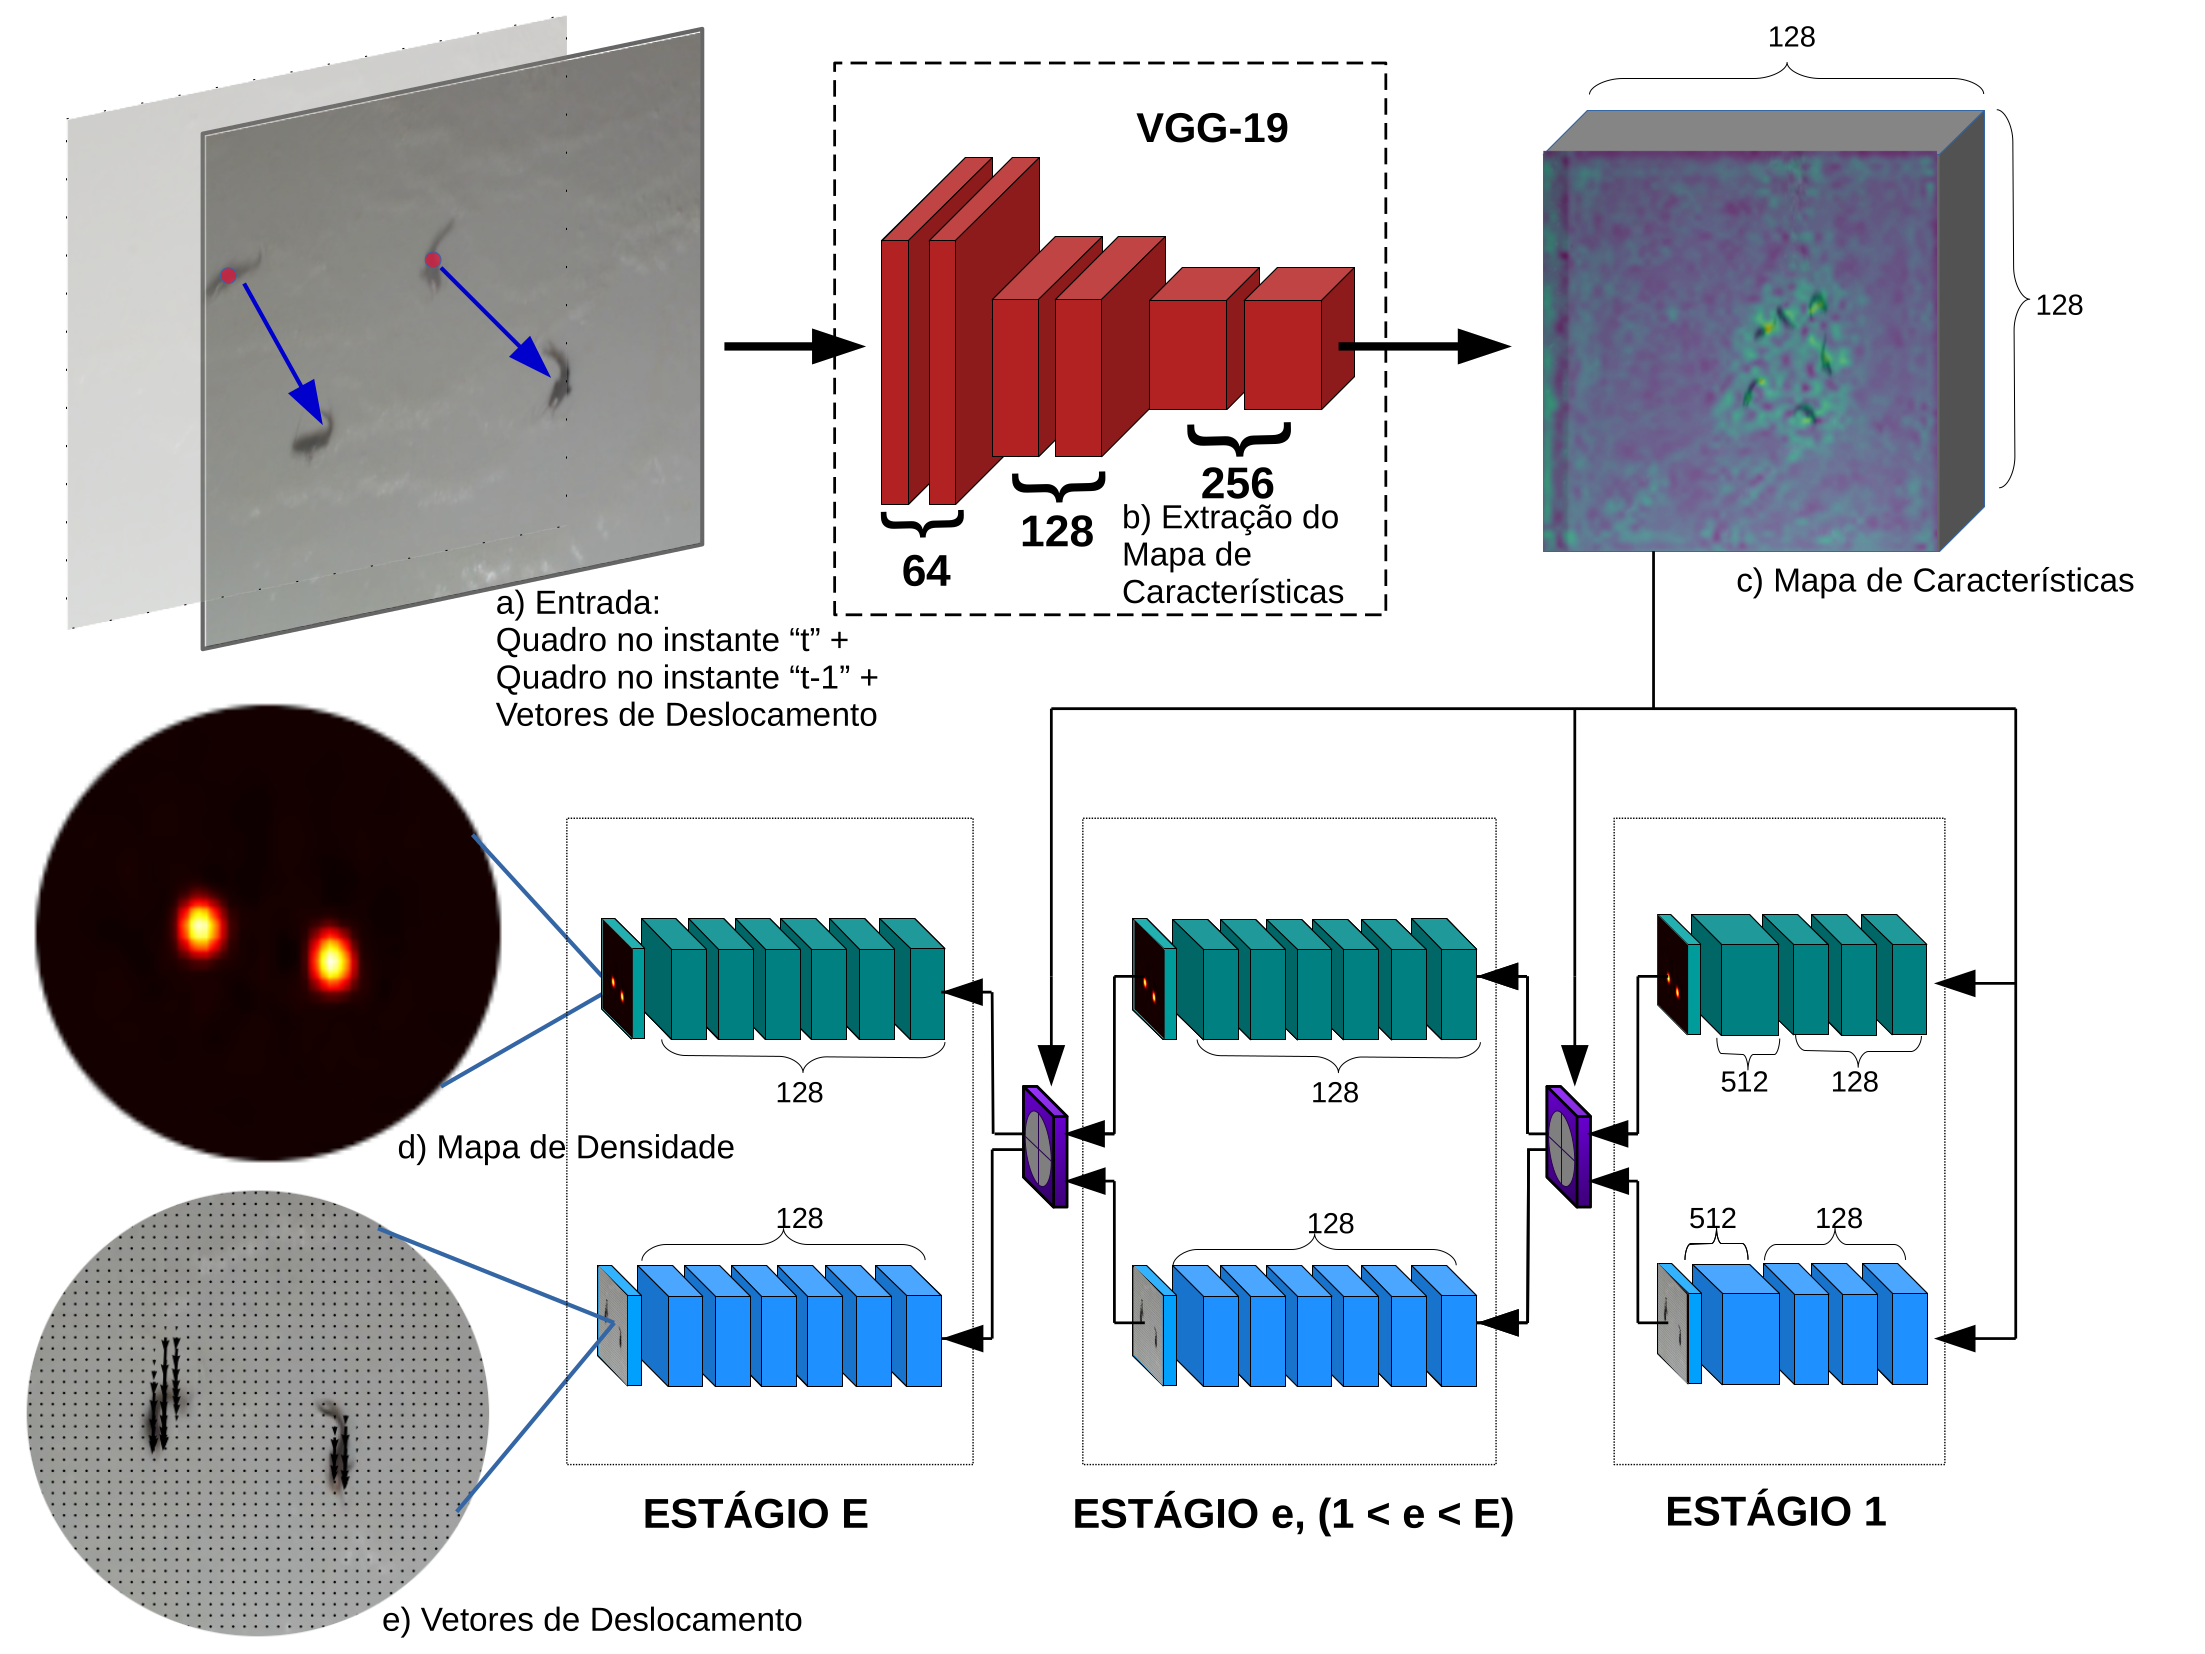
\includegraphics[width=1.06\textwidth]{image/model.png}
	\caption{
	Método proposto recebe o quadro atual $I_{t}$ e o quadro no instante anterior $I_{t-1}$. O resultado da concatenação gera um volume de entrada para a VGG-19. A saída desta arquitetura consiste em um mapa de características inicial. 
	Esse mapa alimenta dois ramos que são responsáveis por realizar as predições do mapa de densidade e de vetores de deslocamento. Cada ramo é composto por uma série de $E$ estágios que refinam a suas predições.
	%Os estágios são as etapas pelas quais o refinamento do mapa de densidade acontece. Cada estágio abrange dois ramos por vez e o resultado de um estágio contém uma grande participação na entrada dos estágios subsequentes. 
	%O mapa de características inicial serve as entradas do estágio 1 até o estágio e. 
	%Os dois ramos de camadas convolucionais são os responsáveis para um melhor ajuste ao modelo: um produz o 1) mapa de densidade e outro os 2) vetores de deslocamento.
	Ambos ramos compartilham as informações para auxiliar na estimação.}
	\label{fig:model} 
\end{figure}
\newpage
\section{Pré-Processamento das Imagens}
\label{sec:Images}

Dada uma imagem $I_t$ no instante $t$ com $w \times h$ pixels, em que $w$ é a largura e $h$ é a altura da imagem, o primeiro pré-processamento consiste em redimensionar todas as imagens para um tamanho fixo de $n \times n$ pixels.
%Em seguida, uma borda de 30 pixels em cada lado da imagem é aplicado.
%Desta forma, um recorte é realizado nas bordas e os peixes são contabilizados apenas na imagem resultante \ref{fig:entrada1}.

%\begin{figure}[!htb]
%	\centering
%	\includegraphics[width=1.0\textwidth]
%	{image/janela2.pdf}
%	\caption{Exemplificação do pré-processamento realizado em cada quadro. Uma borda de 30 pixels em cada lado da imagem é aplicado e os peixes cuja as posições estejam dentre os limites da imagem resultante são contabilizados pelo método.}
%	\label{fig:entrada1} 
%\end{figure} 
%Os ramos são os conjuntos de camadas pelas quais cada $VE$ passa para extração de características. 
%Tendo suas rotinas realizadas por estágios, foram denominados estágio "1", "e = (1<e<E)" e "E". 
%Cada estágio abrange dois ramos, o responsável por extrair os atributos principais dos objetos e o que estima os vetores de deslocamento.
%O mapa de características inicial serve as entradas desde o estágio 1 até o estágio e. 
O método recebe um volume de entrada $V$, resultante da concatenação de um quadro $I_{t}$ no instante $t$ e o quadro anterior $I_{t-1}$, $V = (I_{t},I_{t-1})$, conforme a figura \ref{fig:entrada}.
%o(s) vetor(es) de deslocamento do(s) peixe(s) em um instante anterior $t-1$. 
Sendo $I_{t}$ uma imagem RGB com $512\times512\times3$ pixels e $I_{t-1}$ uma outra imagem do instante anterior com a mesma dimensão, temos que $V$ possui dimensão $ 512\times512\times6$.
%Desta forma temos o volume de entrada $V = (I_{t},I_{t-1})$
%, sendo $I_{t-1}$ os vetores de deslocamento dos peixes de $I_{t-1}$ até $I_{t}$ (Figura \ref{fig:entrada}).
%A CNN VGG-19 (Figura \ref{fig:model}) \cite{VGG} recebe $V$ como entrada e a sua saída consiste em um mapa de características inicial que descreve as informações relevantes da imagem.

\begin{center}
\begin{figure}[!htb]
	\centering
	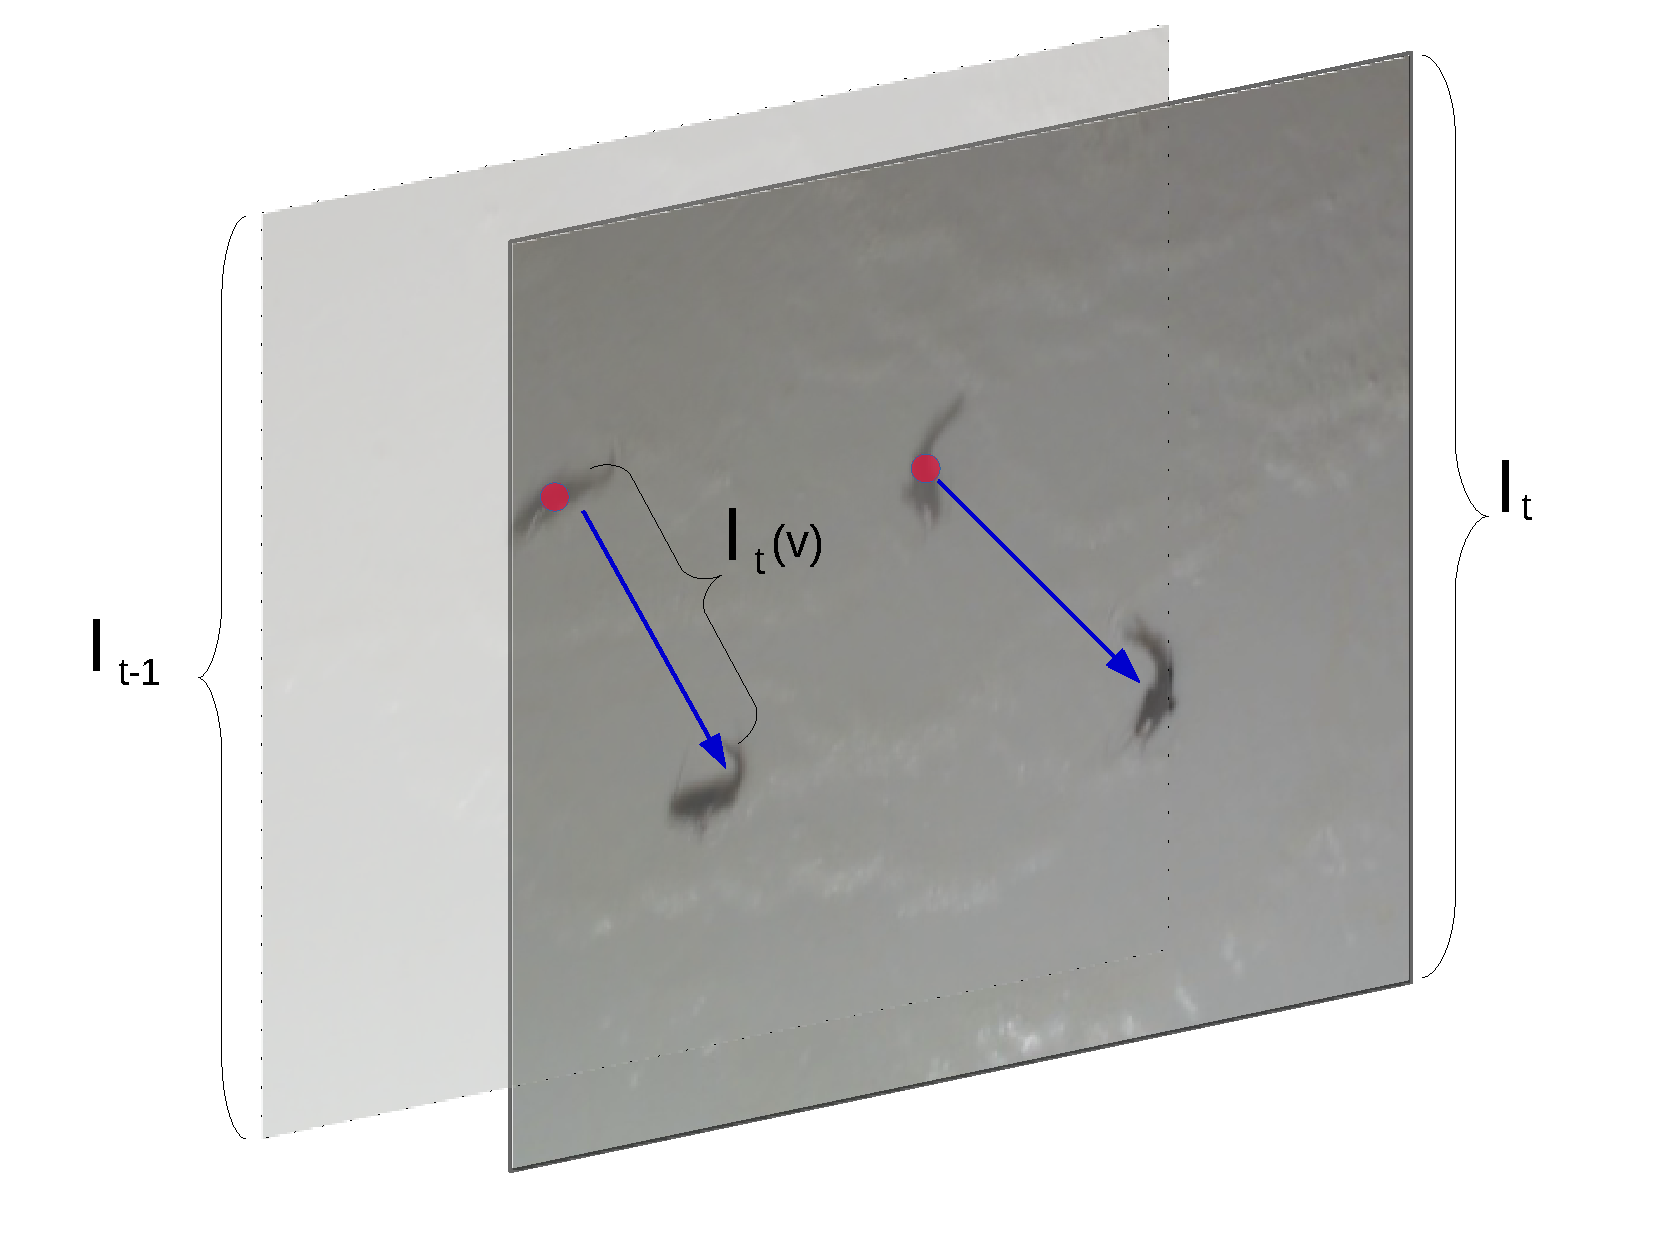
\includegraphics[width=0.9\textwidth]
	{image/VE.pdf}
	\caption{Ilustração do volume de entrada $V$ que consiste na concatenação de um quadro $I_{t}$ e um quadro anterior $I_{t-1}$.}
	\label{fig:entrada} 
\end{figure} 
\end{center}



\section{Extração do Mapa de Características}
   \label{sec:VGG}

Nessa etapa, o volume de entrada $V = (I_{t},I_{t-1})$ é submetido a uma CNN VGGNet \cite{VGG} para obtenção de um mapa de características.
Esse mapa tem como objetivo extrair informações relevantes da imagem de entrada.
A VGGNet mostrou que a profundidade da CNN é um componente importante para o bom desempenho. Os autores da VGG19 apresentaram seis arquiteturas: duas com 11, uma com 13, duas com 16, e uma com 19 camadas \cite{VGG}. A CNN de 19 camadas convolucionais e totalmente conectadas é uma das melhores arquiteturas dentre as propostas pelos autores, sendo uma arquitetura homogênea pois só executa convoluções com campo receptivo $3 \times 3$ e subamostragens $2 \times 2$. A Figura \ref{fig:model} ilustra as camadas da arquitetura VGG19 aplicadas no método proposto.

A entrada da VGG19 consiste em duas imagens RGB com dimensão $512 \times 512 \times 6$, que passa por um pré-processamento inicial no qual é realizada a subtração da cor média de todos os pixels da imagem. Esse processo é repetido para todas as imagens que serão usadas para o treinamento da CNN.
As imagens passam pelas camadas convolucionais que aplicam um filtro de tamanho $3 \times 3$, por ser o menor tamanho capaz de aprender características das quatro direções e do centro durante o processo de convolução. 
O passo de deslocamento do filtro convolucional (\textit{stride}) é de 1 pixel.
O preenchimento com zeros ao redor da imagem é realizado de forma a preservar a dimensão da imagem após a convolução, ou seja, para os filtros de tamanho $3 \times 3$ é usado um preenchimento com zeros de tamanho 1.
Além disso, a função de ativação não-linear ReLu é aplicada após cada camada convolucional.

A amostragem descendente (\textit{Pooling}) é feita através de duas camadas de subamostragens distribuídas no corpo da CNN. Assim, nem todas camadas convolucionais são seguidas de camadas de subamostragens. Os autores usam uma camada de subamostragem máxima com campo receptivo $2 \times 2$ e deslocamento de 2 pixels.
Ao final da primeira etapa, o volume de entrada $V$ é representado por um mapa de características $F$ extraído pelas camadas da VGGNet.
Na Figura \ref{fig:carac} temos a imagem original e o mapa de características obtido através da VGG19.

\begin{figure}[!ht]
	\centering
	\subfloat[Imagem Original]{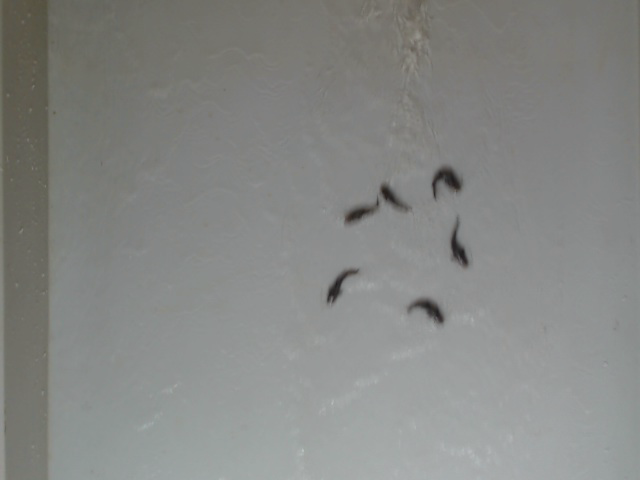
\includegraphics[width=0.5\textwidth]{image/caract.png}}\vspace{0.9cm}
	\subfloat[mapa de características]{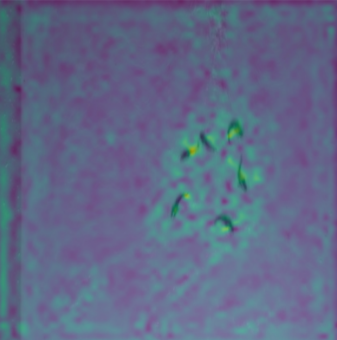
\includegraphics[width=0.37\textwidth]{image/carac.png}}\vspace{0.6cm}
	\caption{\label{fig:carac} Exemplo de um mapa de características predito pela VGG-19.}
\end{figure}  


\section{Estimativa do Mapa de Densidade}
\label{sec:EstimativaDensidade}
Dado o mapa de característica $F$, o primeiro ramo do método proposto estima o mapa de densidade com o objetivo de detectar cada objeto.
Essa predição é realizada por $E$ estágios.
No primeiro estágio (Figura \ref{fig:model} (c)), uma série de camadas convolucionais $\Omega$ geram o mapa de densidade $\hat{C}^1 = \Omega (F)$.
$\Omega$ é uma sequência de cinco camadas convolucionais: três camadas com 128 filtros de tamanho $3 \times 3$, uma camada com 512 filtros de tamanho $1 \times 1$ e uma camada com um único filtro que corresponde ao mapa de densidade.
O segundo ramo responsável pela estimativa dos vetores de deslocamento $\hat{D}^{1}$ estão detalhadas na Seção \ref{sec:EstimativaVetores}. Por enquanto precisamos saber que as estimativas também são utilizados para servir de entrada dos estágios seguintes.

Os estágios refinam as predições do mapa de densidade em etapas sucessivas por $E$ estágios, i.e., $e \in \{1, \dots, E\}$.
Nos estágios subsequentes ao primeiro (Figura \ref{fig:model}), o mapa de características $F$, a estimativa de densidade do estágio anterior $\hat{C}^{e-1}_t$ e as estimativas dos vetores de deslocamento $\hat{D}^{e-1}$ (Seção \ref{sec:EstimativaVetores}) são concatenados e usados para produzir um mapa de densidade refinado $\hat{C}^e = \Psi(F, \hat{C}^{e-1}, \hat{D}^{e-1})$.
A concatenação de diferentes informações auxilia no apendizado do método e espera-se que a informação de deslocamento ajude na detecção dos objetos no quadro atual.
No refinamento, $\Psi$ é uma sequência de sete camadas convolucionais: cinco camadas com 128 filtros de tamanho $7 \times 7$, uma camada com 128 filtros de tamanho $1 \times 1$ e uma camada com um único filtro que corresponde ao mapa de densidade. 



%\begin{figure}[!ht]
%	\centering
%	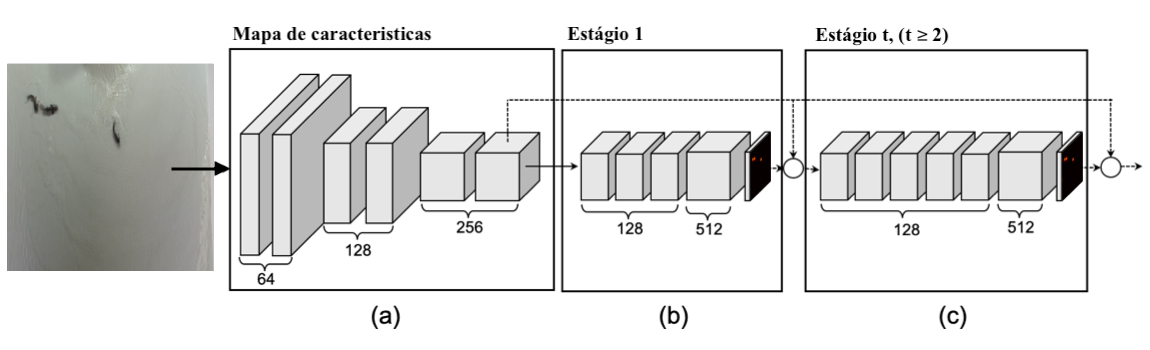
\includegraphics[width=1.0\textwidth]{image/cnn.png}
%	\caption{\label{fig:cnn} CNN usada para predição do mapa de confiança. Bloco inicial (a) é usado para extrair um mapa de recursos da imagem de entrada. Este mapa de recursos é usado como entrada para o primeiro estágio (b). A concatenação do mapa de características e o mapa predito do estágio anterior são usados como entrada para os estágios restantes.}
%\end{figure}  

Para treinar os estágios, a função de perda (Equação \ref{eq:loss}) é aplicada no final de cada estágio comparando a predição do método $\hat{C}^{e}$ com as anotações realizadas por um especialista $C$.
Esta supervisão intermediária aborda o problema do gradiente de desaparecimento, como mostrado em \cite{Cao2017}.
%Como o tamanho do mapa de densidade estimado é menor que o tamanho da imagem, o mapa de densidade \textit{ground truth} é gerado com o tamanho da saída da CNN $[l_F \times l_F]$.

\begin{equation}
f^{e} = \sum_p \parallel C(p) - \hat{C}^{e}(p)\parallel^2_2,
\label{eq:loss}
\end{equation}
onde $C$ é o \textit{ground truth} do mapa de densidade do quadro $t$ gerado de acordo com a Seção \ref{sec:geracao_mapa}. Por fim, a função de perda global é dada pela soma de todos os estágios:

\begin{equation}
f = \sum_{e=1}^{E} f^{e}
\end{equation}

\subsection{Geração do \textit{Ground Truth} do Mapa de Densidade}
\label{sec:geracao_mapa}

Dadas as posições $L = [\{l^1, l^2, \dots, l^K \} \mid \forall \: l^k = (x_k, y_k)]$ de $K$ objetos em um quadro $I_t$, o mapa de confiança (\textit{ground truth}) $C$ é obtido colocando-se um núcleo Gaussiano 2D em cada posição dos objetos. 
Para obter $C$, um mapa de confiança $C^k$ é primeiro calculado para cada objeto $k \in [1, K]$.
O valor de cada posição $p \in \Re^2$ em $C^k$ é definido como:

\begin{equation}
C^k(p) = \exp \left(- \frac{\| p - l^k \|^2_2}{\sigma^2}\right),
\end{equation}
onde $\sigma$ corresponde a largura dos picos que representa cada objeto.
%onde $\sigma = \{\sigma_{min}, \dots ,\sigma_{max}\}$ sendo $\sigma_i \in \mathbb{R}^*_+$. $\sigma_{max}$ aponta a largura da base dos picos e $\sigma_{min}$ recebe um valor mínimo que indica a largura das extremidades. Assim $\sigma$ limita o tamanho dos picos para estimar o tamanho médio de cada objeto.

%\begin{equation}
%    \label{eq:sigma}
%    \sigma = \sum_{i=s_{min}}^{s_{max}} s_{i}
%\end{equation}

%onde $\sigma = \sum_{i=m}^{s_i} s_{max}$ e $s_i \in \mathbb{R}^*_+$.


%Idealmente, $\sigma$ é proporcional à largura média do objeto.
O mapa de confiança $C$ é obtido pela agregação dos mapas individuais via operador máximo:

\begin{equation}
C(p) = \max_{1<k<K} C^k(p).
\end{equation}

A Figura \ref{fig:sigma} ilustra o mapa de confiança para uma imagem e dois valores de $\sigma$.
A primeira imagem mostra as posições dos objetos em pontos vermelhos que foram anotados pelo especialista.
As próximas duas imagens apresentam os mapas de confiança para $\sigma = 1.5$ e $2.5$, respectivamente.
Por fim, usamos o mapa de confiança \textit{ground truth} para treinar a abordagem proposta.

\begin{figure}[!ht]
	\centering
	\subfloat[Imagem Original]{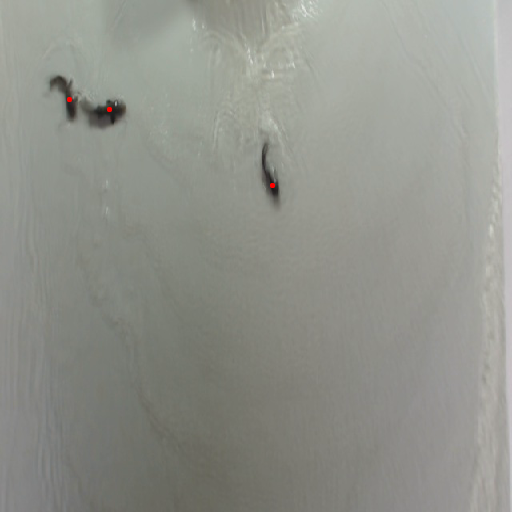
\includegraphics[width=0.3\textwidth]{image/sigmas/frame001018Ponto.png}}\vspace{0.2cm}
	\subfloat[$\sigma = 1.5$]{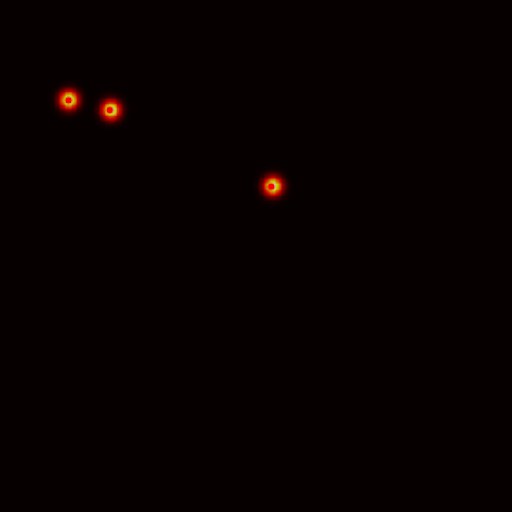
\includegraphics[width=0.3\textwidth]{image/sigmas/frame001018_label_1_5.png}}\vspace{0.2cm}
	\subfloat[$\sigma = 2.5$]{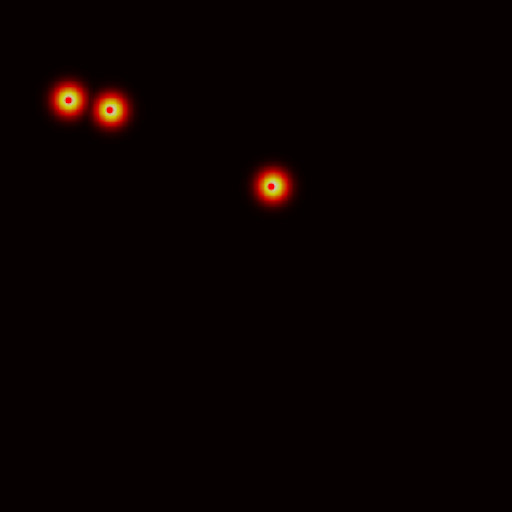
\includegraphics[width=0.3\textwidth]{image/sigmas/frame001018_label_2_5.png}}
	\caption{\label{fig:sigma} Exemplo de uma cena e seu mapa de confiança correspondente para diferentes valores de $\sigma$.}
\end{figure}  


\section{Estimativa dos Vetores de Deslocamento}
\label{sec:EstimativaVetores}

O segundo ramo do método proposto (Figura \ref{fig:model} (d)) possui camadas convolucionais com os mesmos parâmetros do primeiro ramo.
%Entretanto, a útilma camada de cada estágio produz um vetor un
Entretanto, a última camada de cada estágio produz a estimativa do deslocamento em x e y.
O primeiro estágio possui uma série de camadas convolucionais $\Omega$ que geram os vetores de deslocamento $\hat{D}^{1} = \Omega (F)$ para o quadro $t$.

Nos demais estágios, o mapa de características $F$, o mapa de densidade $\hat{C}^{e-1}$ (Seção \ref{sec:EstimativaDensidade}) e a estimativa do estágio anterior $\hat{D}^{e-1}$, são concatenados e usados para produzir os vetores de deslocamento refinado $\hat{D}^{e} = \Psi(F,\hat{C}^{e-1}, \hat{D}^{e-1}$). 
$\Psi$ é uma sequência de sete camadas convolucionais conforme o primeiro ramo.

Para treinar os estágios dos vetores de deslocamento, a função de perda (Equação \ref{eq:loss2}) é aplicada no final de cada estágio.

\begin{equation}
f^{e} = \sum_p \parallel D(p) - \hat{D}^{e}(p)\parallel^2_2,
\label{eq:loss2}
\end{equation}
onde $D$ é o \textit{ground truth} dos vetores de deslocamento do quadro $t$ gerado de acordo com a Seção \ref{sec:geracao_mapa2}. Por fim, a função de perda global é dada por:

\begin{equation}
f = \sum_{e=1}^{E} f^{e}
\end{equation}

\subsection{Geração do \textit{Ground Truth} do Vetor de Deslocamento}
\label{sec:geracao_mapa2}

%Dada a posição $l^k_t \in L$ (Seção \ref{sec:geracao_mapa}) de um objeto $k$ presente em um quadro $t$, campos vetoriais são estimados, onde $l_{t,n} \in \mathbb{R}^{w\times h\times2}$, $f \in \{1...N\}$, cada local da imagem em $L_t$ codifica um vetor 2D.

Considere $l_t^k$ como a posição de um objeto $k$ no quadro $t$ e $l_{t-1}^k$ sua posição no quadro anterior.
%Considere a posição de um objeto k na imagem como $l_t^k$ e a sua posição no quadro anterior  
O vetor de deslocamento do objeto $k$ é um vetor que aponta de $l^k_{t-1}$ até $l^k_{t}$, conforme a Figura \ref{fig:vetor}.
Para a construção dos vetores de deslocamento densos, isto é, para cada pixel da imagem, um conjunto de pixels $\rho$ ao redor do vetor de deslocamento principal é obtido.
Todos os pixels cuja a distância para o vetor de deslocamento for menor ou igual a um é considerado nesse conjunto.
%Considere a posição de um único objeto presente em um quadro, sendo $x_{i2}$ o \textit{Ground Truth} e a posição de onde ele se encontrava no quadro anterior sendo $x_{i1}$. 
%Sendo $\rho$ o conjunto de pixels referentes a $l^k_{t}$. 
Cada pixel $p \in \rho$ armazena um vetor unitário $v$ com a mesma direção do deslocamento de $t-1$ para $t$ do objeto $k$, sendo $v = (l^k_{t-1} - l^k_{t})/\|(l^k_{t-1} - l^k_{t})\|_2$.
Os pixels restantes recebe um vetor nulo. 
O mesmo procedimento é realizada para todos os objetos $k$ no quadro atual e um mapa denso de vetor de deslocamento $D$ é obtido para treinamento do método proposto.

\begin{figure}[!htb]
	\centering
 	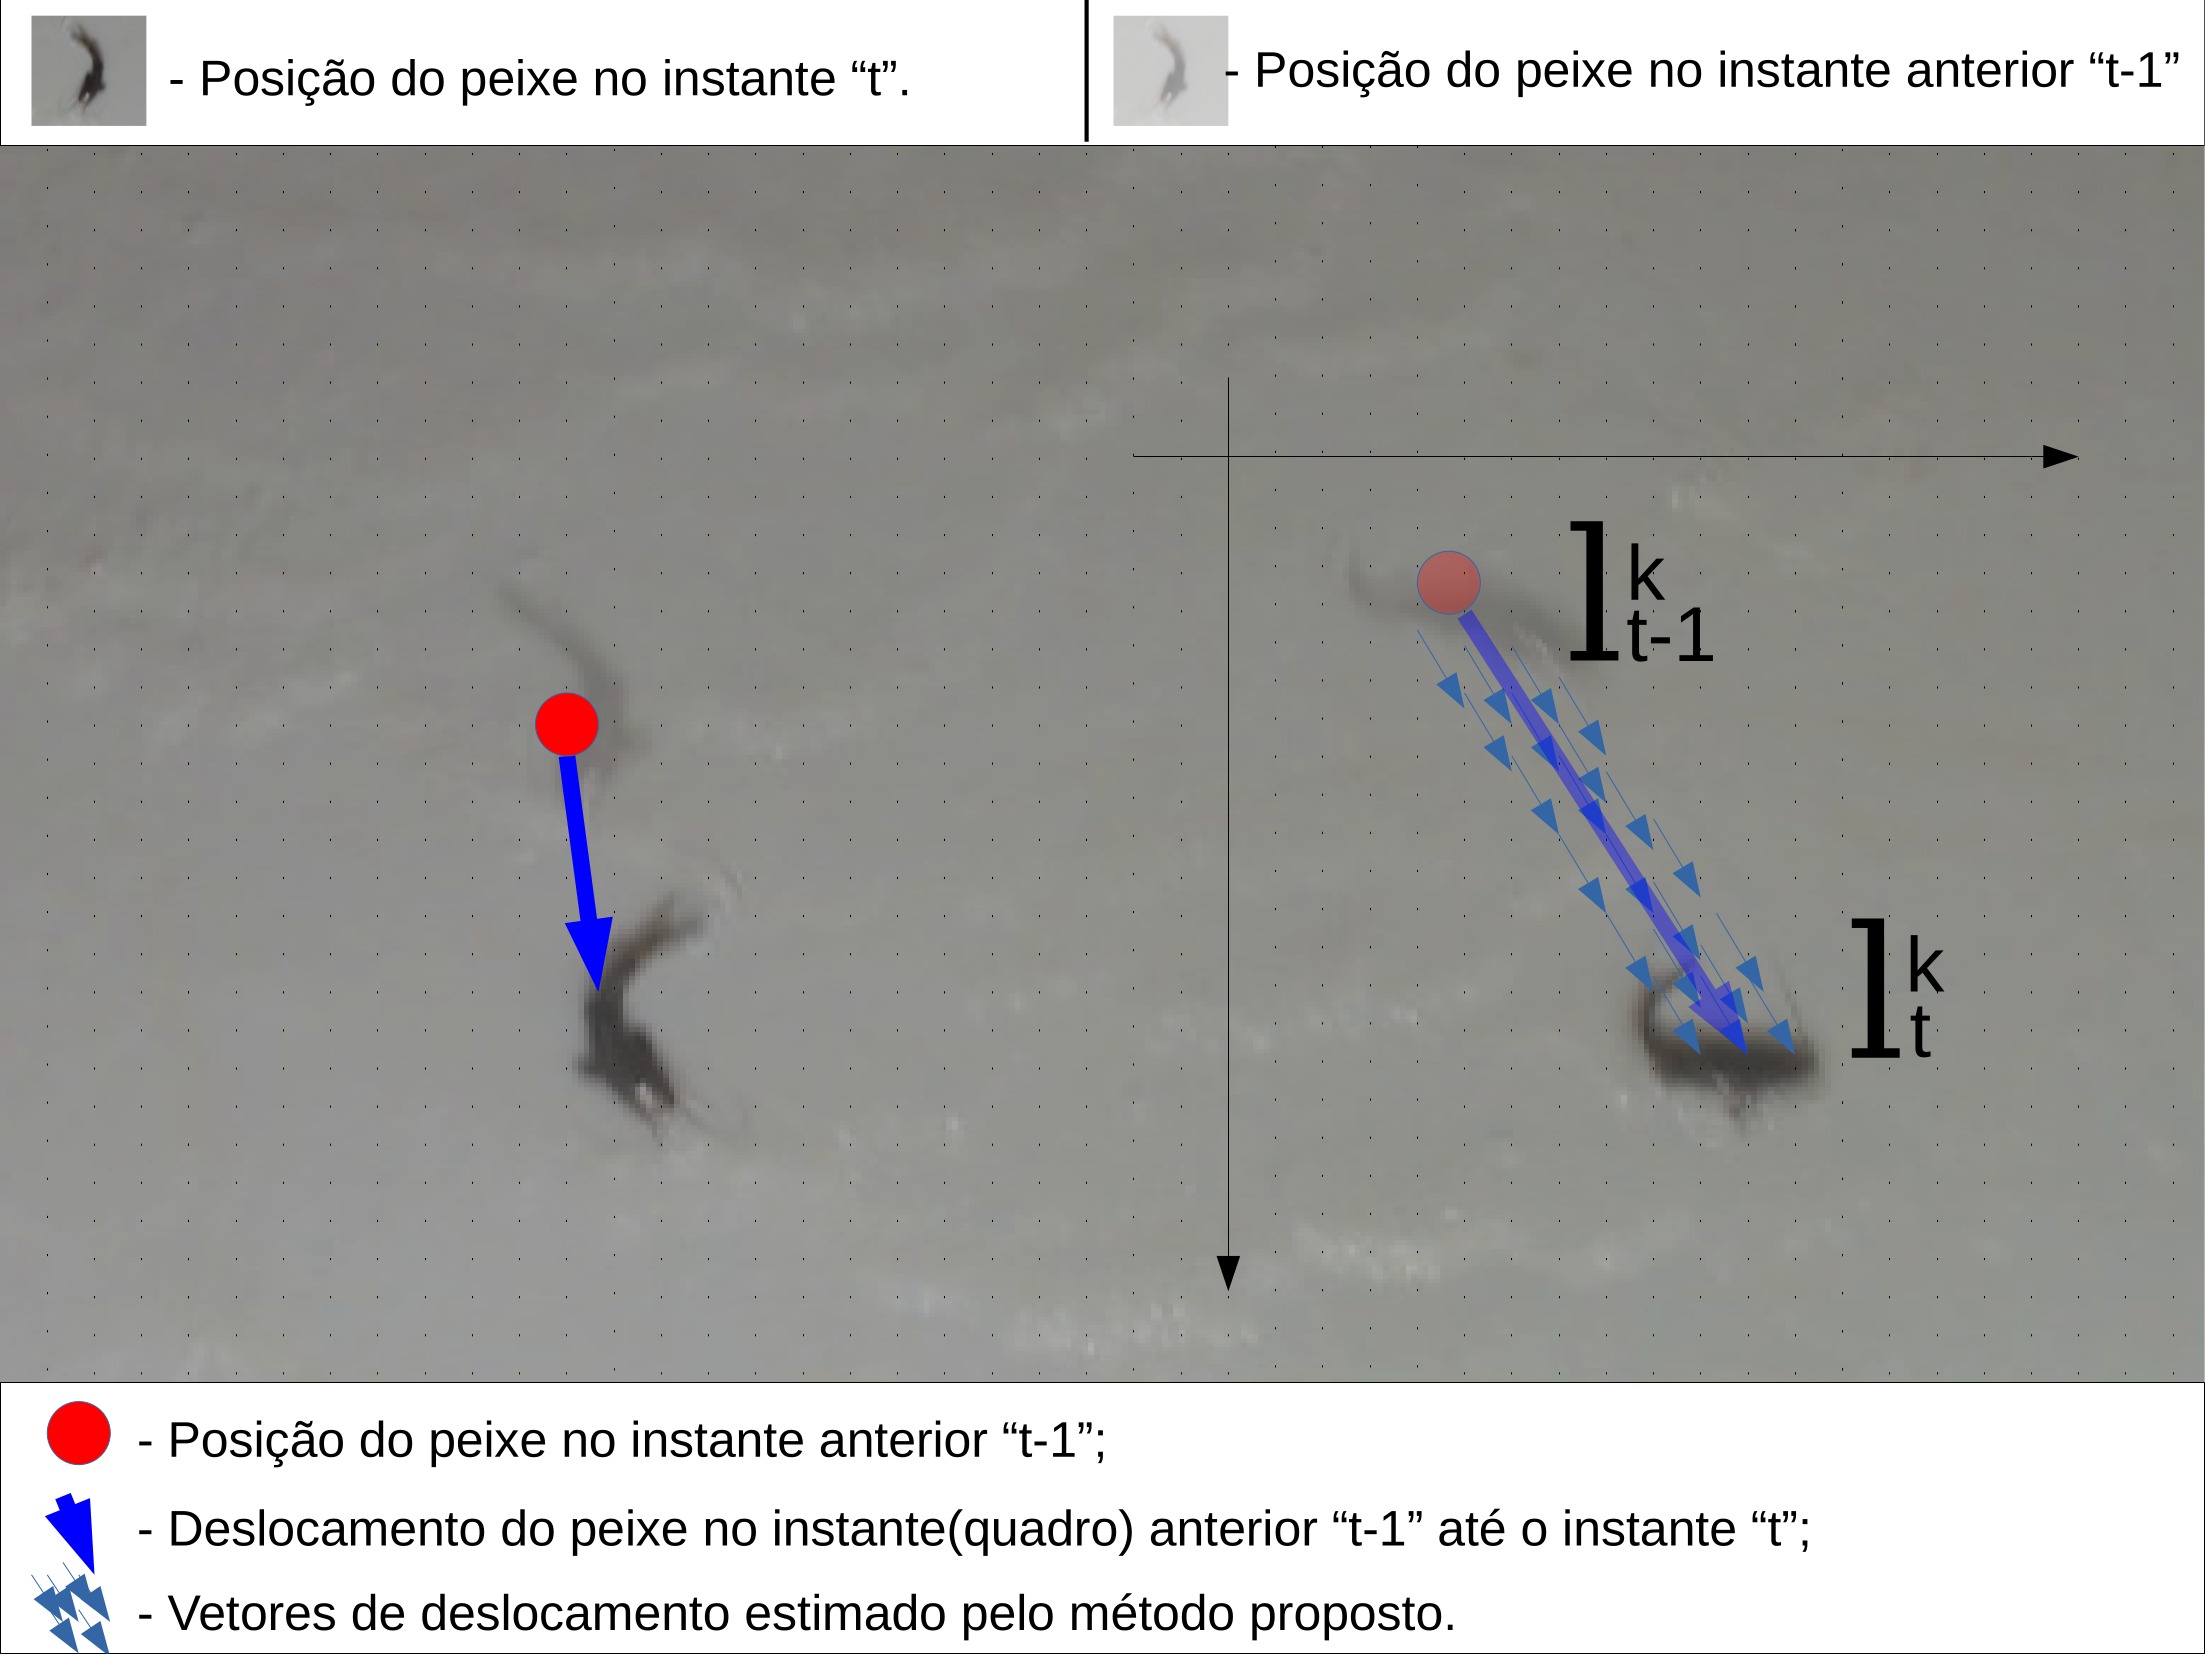
\includegraphics[width=.9\textwidth]{image/VD.png}\vspace{0.2cm}
	\caption{\label{fig:vetor} Ilustração de um vetor para um objeto em quadro.}
\end{figure} 


A Figura \ref{fig:vetores} mostra os alevinos na cor branca, os pontos na cor azul apontam a posição dos alevinos no quadro atual $I_t$ e os pontos na cor vermelho mostram as localizações no quadro anterior $I_{t-1}$. Nas imagens da Figura \ref{fig:vetores2} temos a ilustração dos vetores estimados, sendo estimado um vetor para cada pixel que representa o objeto de interesse.
%As figuras mostram os pontos do quadro anterior quando apenas dois \textit{frames} são utilizados, quando o número de quadros anteriores é superior a um, os quadros atuais apontam um vetor com as posições anteriores de cada filhote.

\begin{figure}[h]
	\centering
	\subfloat[]{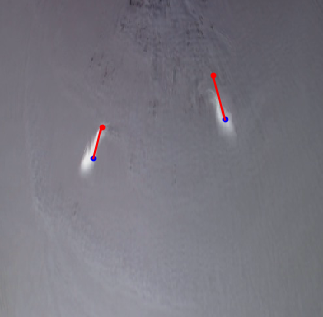
\includegraphics[width=0.3\textwidth]{image/frame000089.png_tracking.png}}\vspace{0.1cm}
	\subfloat[]{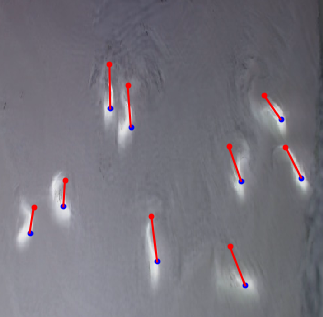
\includegraphics[width=0.3\textwidth]{image/frame000126.png_tracking.png}}\vspace{0.2cm}
	\subfloat[]{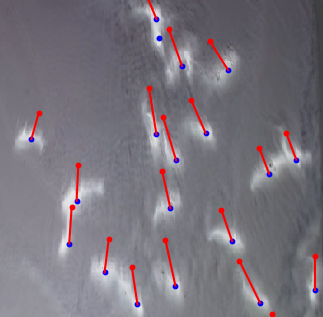
\includegraphics[width=0.3\textwidth]{image/frame000176.png_tracking.png}}
	\caption{\label{fig:vetores} Exemplos das localizações nos vetores}
\end{figure} 

\begin{figure}[h]
	\centering
	\subfloat[]{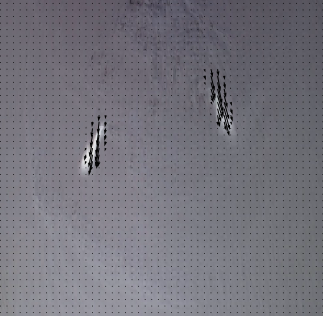
\includegraphics[width=0.3\textwidth]{image/frame000089.pngquiver_t.png}}\vspace{0.1cm}
	\subfloat[]{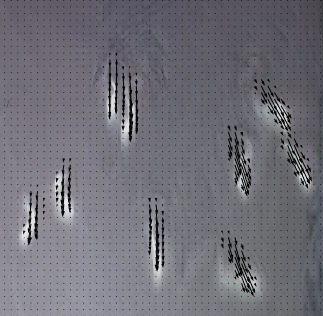
\includegraphics[width=0.3\textwidth]{image/frame000126.pngquiver_t.png}}\vspace{0.2cm}
	\subfloat[]{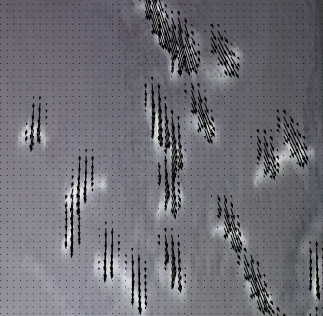
\includegraphics[width=0.3\textwidth]{image/frame000176.pngquiver_t.png}}
	\caption{\label{fig:vetores2} Ilustração dos vetores estimados pelo segundo ramo apresentado, para cada pixel de cada objeto.}
\end{figure} 

\newpage
\section{Localiza\c{c}\~{a}o dos Objetos pelo Mapa de Densidade}

A localização dos objetos é obtida dos picos (máximo local) do mapa de densidade predito do último estágio $\hat{C^E}$.
Um local $p=(x_p, y_p)$ é um máximo local se $\hat{C^E}(p) > \hat{C^E}(v)$ para todos os vizinhos $v$.
Consideramos a vizinhança de 4 pixels para todos os locais $p = (x_p, y_p)$, ou seja, $v = (x_p \pm 1, y_p)$ ou $(x_p, y_p \pm 1)$.

Para evitar ruído, os picos precisam ser separados por pelo menos $\delta$ pixels.
Isso impede que dois alevinos sejam detectados muito próximos uns dos outros.
Além disso, um pico deve ter uma confiança maior que um limite $\tau$.
Após experiências preliminares, usamos $\delta = 10$ e $\tau = 0.2$.
A Figura \ref{fig:heatmap} mostra um exemplo tridimensional do mapa de confiança, onde a largura e a altura são as dimensões da imagem e os picos azuis representam as regiões com máxima confiança local.

\begin{figure}[h]
	\centering
	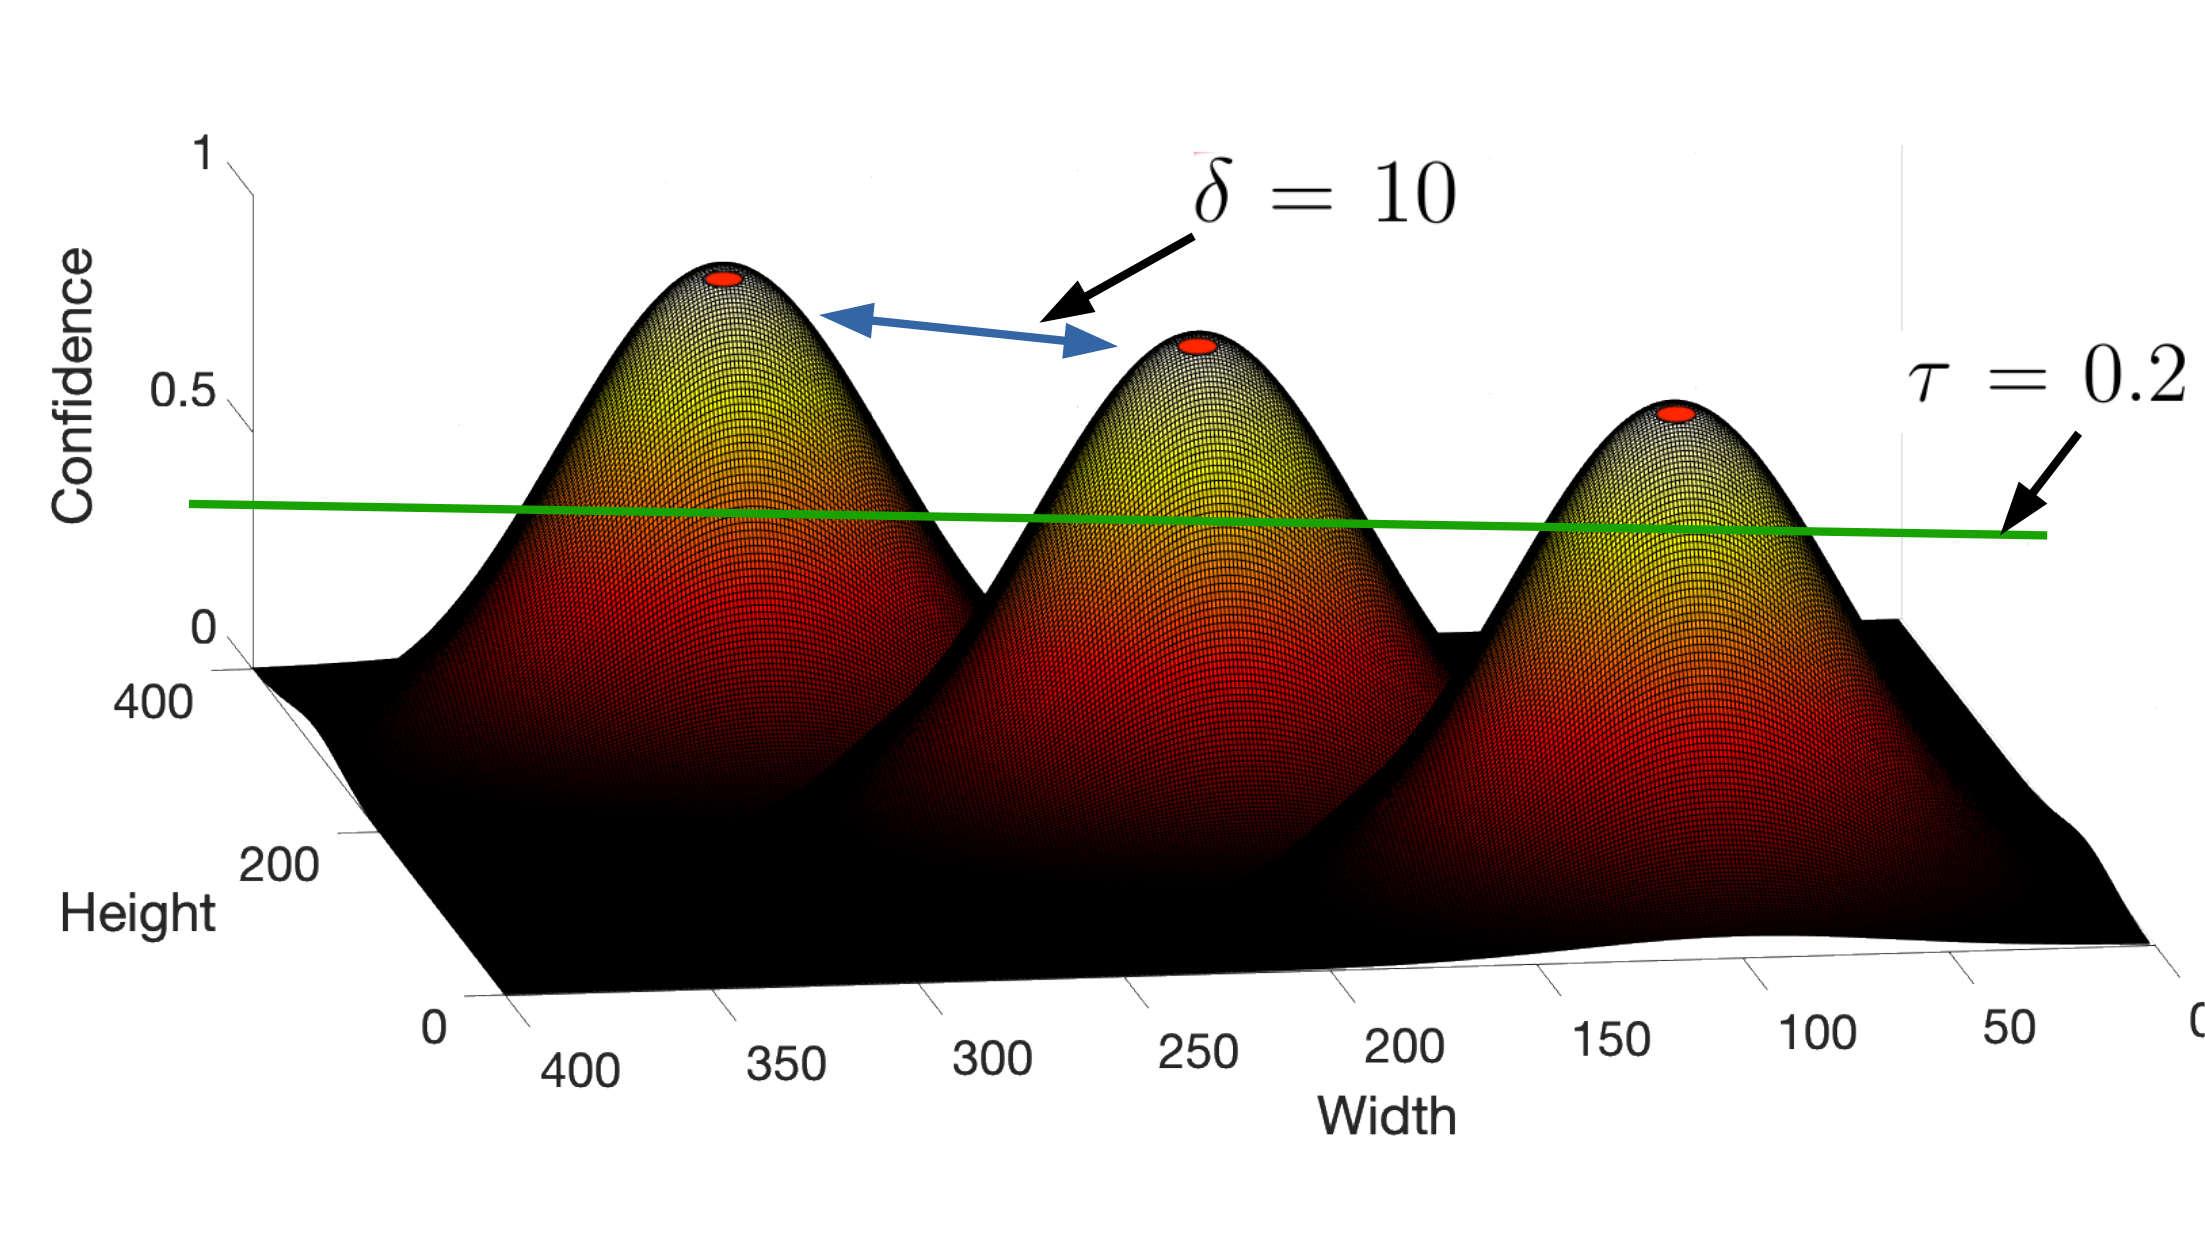
\includegraphics[width=.6\columnwidth]{image/heatmap2.png}
	\caption{Exemplo do mapa de confiança em três dimensões.}
	\label{fig:heatmap}
\end{figure}  

\label{chap:ranking}

   \chapter{Experimentos e Resultados}
    \label{chap:experimentos}
   \section{Base de Imagens}
    \label{chap:basedeimagens}
   
   Os vídeos aplicados nos experimentos foram obtidos a partir do banco FISHCV155V, desenvolvido pelo grupo INOVISÃO da UCDB, em parceria com o IFMS e a empresa Projeto Pacu  \cite{Junior2019UFMS}. Os vídeos foram gravados entre os meses de julho e setembro de 2018 com uma câmera com resolução full hd ($1920\times1080$ pixels) e uma taxa de captura de 30 quadros por segundo. A câmera foi acoplada a uma estrutura criada pelos autores com uma inclinação aproximada de 12 graus, por onde os alevinos deslizam com o auxílio de água. A Figura \ref{Estrutura} mostra a estrutura construída para a obtenção dos vídeos.
   
   \begin{figure}
	\noindent\makebox[\textwidth]{%
		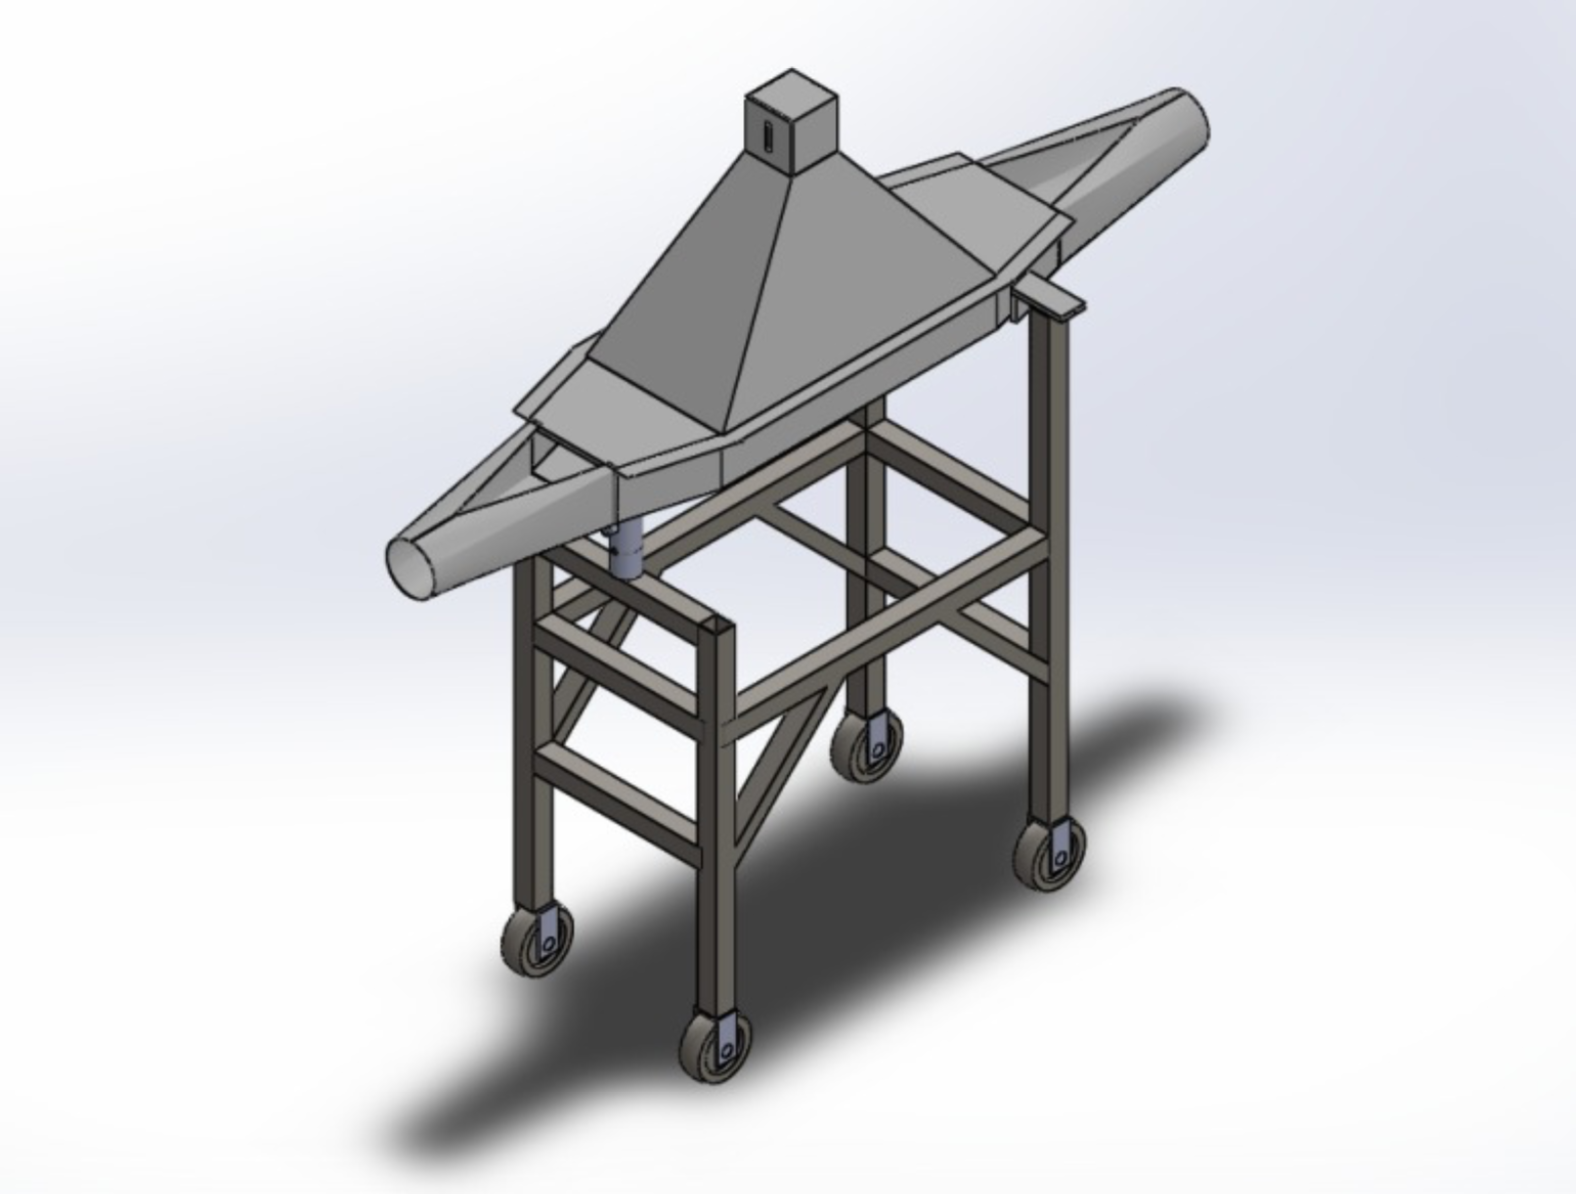
\includegraphics[width=0.5\textwidth]{image/estruturaCaptura.png}}
	\caption{Suporte para Captura das imagens proposta por \cite{Junior2019UFMS}}
	\label{Estrutura}
    \end{figure}
   
   Dentre os vídeos do banco de dados FISHCV155V, foram selecionados aleatoriamente 15 para compor o banco de dados do experimentos.
   O conjunto de treinamento é composto por 7 vídeos, sendo que o menor (tempo) vídeo contém 180 quadros e o maior 750 quadros; O conjunto de testes possui 4 vídeos, entre 240 e 300 quadros. %o menor contém 240 quadros e o maior contém 300; 
   O conjunto de validação possui 4 vídeos, sendo o menor 210 quadros e o maior 390. Na Figura \ref{Train} temos alguns exemplos das imagens utilizadas nos experimentos.
   Na Tabela \ref{tab:separation} a quantidade exata do conjunto é apresentado.
   
    \begin{table}[htb]
	\centering	
	\begin{tabular}{|p{2.7cm}|c|c|}
		\hline
		\multirow{2}{\linewidth}{\centering \textbf{Banco de Dados}} & \multicolumn{2}{|c|}{\textbf{Quantidades}} \\
    	\cline{2-3}
    	  & \textbf{Vídeos} & \textbf{Quadros} \\
		\hline
		Treinamento & $7$ & $2730$\\
		\hline
		Teste & $4$ & $1080$ \\
		\hline
		Validação & $4$ & $1230$ \\
		\hline
	\end{tabular}
	\caption{\label{tab:separation} Separação dos vídeos e quadros para os Experimentos}.
    \end{table}

   \begin{figure}[htb]
		\centering
		%\textbf{SEGNET SEM PONDERAÇÃO - OLHO DE RÃ} \\
		\subfloat{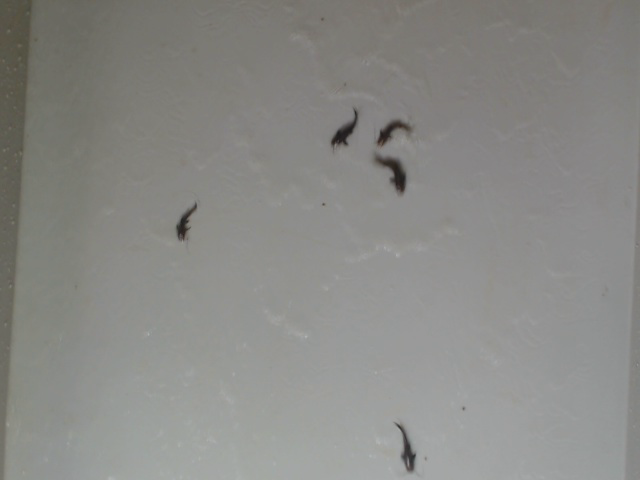
\includegraphics[width=.32\columnwidth]{image/Train/VID15_frame000222.png}}
		\hspace{.1cm}
		\subfloat{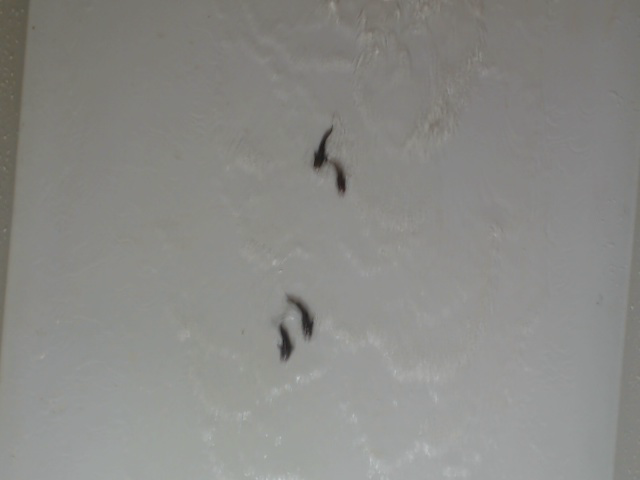
\includegraphics[width=.32\columnwidth]{image/Train/VID18_frame000244.png}}
		\hspace{.1cm}
		\subfloat{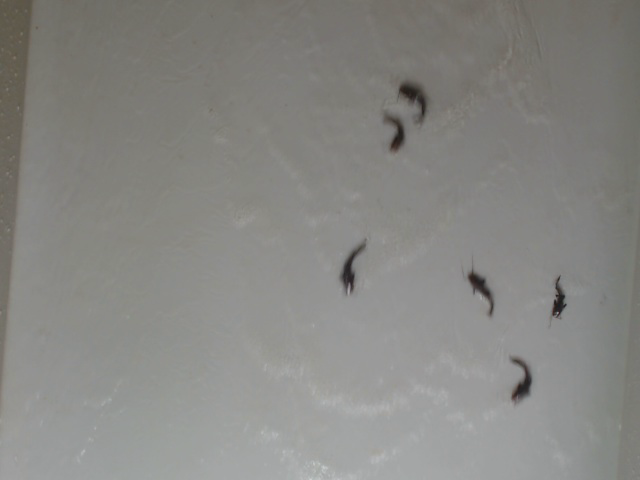
\includegraphics[width=.32\columnwidth]{image/Train/VID19_frame000313.png}}
		\hspace{.1cm}
		\caption{Imagens retiradas do conjunto de Treinamento \cite{Junior2019UFMS}.} % caption for whole figure
		\label{Train}
	\end{figure}
	


\subsection{Configuração dos Experimentos}

Para avaliar a abordagem proposta, as amostras foram divididas aleatoriamente em conjuntos de treinamento contendo 7 vídeos, validação 4 vídeos e teste 4 vídeos.
Para o treinamento, o otimizador Gradiente Descendente Estocástico foi usado com um momento de 0,9.
O ajuste de hiper parâmetros na taxa de aprendizado e no número de épocas foi realizado usando o conjunto de validação para reduzir o risco de \textit{overfitting}.
Após experimentos preliminares para ajuste de hiper parâmetro, a taxa de aprendizado foi de 0,01 e o número de épocas foi de 100.

Todos os experimentos foram executados na GPU (Unidade
de Processamento Gráfico) NVIDIA GeForce GTX TITAN X (5120 Compute Unified Device Architecture - núcleos CUDA e memória gráfica de 12 GB ), sistema operacional Ubuntu 18.04. A implementação proposta faz o uso da API (Interface de Programação de Aplicativos) de alto nível denominada Keras \cite{chollet2015keras}, escrita na linguagem de programação Python. As rotinas desta interface são executadas através da biblioteca de código aberto TensorFlow \cite{tensorflow2015-whitepaper}.

\subsubsection{Transfer Learning}
Em vez de treinar a abordagem proposta do zero, os pesos da primeira parte foram inicializados com pesos pré-treinados no ImageNet em um conceito conhecido como \textit{transfer learning}.
Esse método proporciona uma certa rapidez no treinamento de CNNs, evitando treinamentos do zero (aleatoriamente). 
Quanto maior e mais geral o conjunto de treinamento do modelo pré-treinado, maior será a eficiência da transferência de aprendizado (\cite{tensorflow2015-whitepaper,c231stan}). 
A ImageNet é um conjunto que contém 1,2 milhões de imagens com 1000 categorias \cite{DBLP:journals/corr/RussakovskyDSKSMHKKBBF14}. Por ser um conjunto extenso existem vários modelos treinados nas arquiteturas mais conhecidas da literatura.

\subsubsection{Métricas de Classificação}
%\paragraph{MAE}
Para avaliar o método foram utilizados as métricas de regressão que medem a concordância entre o número de objetos anotados e os preditos. A métrica de erro absoluto médio (\textit{mean absolute error} - MAE) é calculada conforme a Equação \ref{eq:MAE}.

\begin{equation}
\label{eq:MAE}
    MAE = \frac{\sum^{T}_{t=1}{|\hat{x}_t-{x}_t|}}{T}
\end{equation}
onde $\hat{x}_t$ representa o número de objetos preditos pelo método e ${x_t}$ o número de objetos anotados em um conjunto de $T$ quadros do conjunto de testes \cite{MAE}. 

%, erro quadrático médio (\textit{mean squared error} - MSE) 
%,coeficiente de determinação ($R^2$) e erro quadrático médio da raiz normalizado (\textit{normalized root-mean-squared error} - NRMSE).

Para avaliar a localização dos objetos preditos em uma imagem, nós usamos a precisão, revocação e métrica F1 ou medida-f.
Para calcular essas métricas, é necessário determinar o número de verdadeiros positivos (VP), falsos positivos (FP) e falsos negativos (FN).
Um verdadeiro positivo é obtido se um ponto predito pelo método proposto está dentro de um raio máximo $r$ de um ponto rotulado (neste trabalho usamos raio máximo igual a 5 pixels).
Um falso positivo é obtido quando o método proposto prediz um objeto que não foi rotulado, isto é, nenhum ponto a uma distância $r$.
Por fim, um falso negativo é obtido quando nenhum ponto é predito a uma distância $r$ de um ponto rotulado.

A Precisão é definida conforme a Equação \ref{eq:precision}, isto é, o número de verdadeiros positivos (VP) sobre o número de verdadeiros positivos mais o número de falsos positivos (FP).

\begin{equation}
\label{eq:precision}
    P = \frac{VP}{VP+FP}
\end{equation}

Revocação é definido com o número de verdadeiros positivos (VP) sobre o número de verdadeiros positivos mais o número de falsos negativos (FN), conforme a Equação \ref{eq:recall}.

\begin{equation}
    \label{eq:recall}
    R = \frac{VP}{VP+FN}
\end{equation}

Para obter uma exatidão dos acertos, usamos a F1 que produz uma média harmônica da precisão e da revocação. A revocação está focada nos pontos que deverão ser classificados como positivos, enquanto que a precisão calcula os pontos positivos que foram preditos como positivos pelo modelo. A função alcança seu melhor valor em 1 e pior em 0 \cite{f1}: 
\begin{equation}
    F1 = 2 \cdot \frac{P\cdot R}{P + R}
\end{equation}


\section{Resultados e Discussão}
\label{sec:resultados}
%Tendo $n$ peixes no conjunto de testes para ser contados, os resultados a seguir apresentam a performace do método para a contagem de todos os peixe e em quadros que possuem $n$ peixes ou mais. Assim são apresentados os resultados para $n \geq \{1,2,4,6,8,10\}$ peixes, o acumulo de estágios e a utilização ou não do vetor de deslocamento no volume de entrada.


Nas subseções abaixo são demonstrados os resultados com detalhes condizente com os experimentos e as técnicas que geraram resultados relevantes.

\subsection{Resultados Quantitativos}
\label{subsec:ResultadosQ}
As Tabelas \ref{tab:resultadosGeral}, \ref{tab:resultadosEstagios} e \ref{tab:resultadosTemporal} mostram os resultados obtidos nos experimentos do método proposto após treinamentos de 100 épocas.
As tabelas apresentam a comparação dos resultados obtidos para diferentes variações de sigmas, número de estágios e o uso dos vetores de deslocamento como informação auxiliar na detecção dos objetos. 
Para uma avaliação adequada em desafios com vários peixes em um único quadro, nós reportamos as métricas em diversos cenários apresentados em cada coluna nas tabelas.
O primeiro considera o cálculo das métricas em todos os quadros do conjunto de teste (primeira coluna das tabelas).
Os demais cenários consideram somente quadros que contenham uma quantidade $i$ de peixes, e $i \geq {1,2,4,6,8,10}$.
%Os demais cenários consideram somente quadros com uma certa quantidade de peixes.
Por exemplo, a coluna $i \geq 10$ indica que somente foram considerados os quadros com 10 ou mais peixes no cálculo das métricas.
Portanto, o desafio imposto nesse cenário é muito maior quando comparado com quadros com poucos peixes.

%Para avaliar a quantidade de peixes contados em cada quadro, temos um comparativo referente a quantidade de peixes presentes em uma imagem. Desta forma os resultados apresentados se dão para os quadros que possuem uma quantidade $ i \geq  \{1,2,4,6,8,10\}$ de peixes.
%, o acumulo de estágios e a utilização ou não do vetor de deslocamento no volume de entrada
%Em negrito apresentam o melhor resultado.

%A contabilização dos quadros que contém a quantidade de peixes $\leq 6$, apresentam valores notoriamente inferiores para a função de erro $MAE$, em sua maioria os resultados são $\leq 1$ e muito próximos de 0. Por outro lado, a partir de 6 peixes na imagem a função alcança valores $\geq 1$. O teste com todos os quadros, por consequência todos os peixes $MAE = 0.116$ conforme a Tabela \ref{tab:resultadosGeral}.

%Em geral $R^2$ aponta valores inferiores quando a arquitetura não se adapta ao conjunto de dados, o melhor resultado obtido alcançou 94.1\%, que afirma o ajuste do modelo ao conjunto de dados. 
Conforme descrito da Seção \ref{sec:geracao_mapa}, a parâmetro $\sigma$ controla a largura dos picos que representa cada objeto no mapa de densidade.
Isto posto, a Tabela \ref{tab:resultadosGeral} apresenta os resultados dos experimentos realizados para uma variação do valor de $\sigma$.
Dessa forma, $\sigma = 0.7$ gera picos com um raio menor, enquanto $\sigma = 1.3$ gera picos com um raio maior. 
O número de estágio nesses experimentos foi fixado em $E = 4$.


%Ainda na Tabela \ref{tab:resultadosGeral}, temos um comparativo dos resultados obtidos, para cada valor de sigma, e a quantidade de peixes a serem contados em cada quadro. 
%Os valores exibidos apontam que quanto menor o valor de sigma, menor será os valores resultantes.
%Especialmente quando há uma quantidade significativa de peixes presentes é levado em consideração.


Analisando os resultados apresentados na Tabela \ref{tab:resultadosGeral}, podemos notar que o melhor resultado foi obtido para $\sigma = 1.1$, alcançando $F1 = 98\%$ e $MAE = 0.11$ de acertos e erros contabilizando todos os quadros.
Esse resultado é extremamente relevante pois o método proposta erra em média apenas 0.11 peixes por quadro.
Como esperado, quando a quantidade de peixes considerados por quadro aumenta, os valores de acertos diminuem.
Entretanto, mesmo quando somente quadros com 10 ou mais peixes são considerados, foram obtidos resultados relevantes com $F1 = 90\%$ e MAE = 1.71.
Para as variadas quantidade de peixes $\geq 1,2,4,6,8,10$ o melhor $\sigma$ obteve uma média de $F1 =  93\%$ de acertos.

%, valores presentes na Tabela \ref{tab:resultadosGeral}.

%dentre eles está a utilização dos 2 quadros processados, sendo 1 o quadro atual e 2 quadros anteriores para adquirir o deslocamento dos alevinos. Com a ciência da localização em 3 \textit{frames}, a função $F1$ aponta 96.8\% de acertos entre os Verdadeiros Positivos e os Falsos Positivos $\sigma_{max}$ = 3.0 e $\sigma_{min}$ = 1.5(Seção \ref{sec:geracao_mapa2}) conforme ilustrado na Tabela \ref{tab:resultados3} . O resultado que mais se destacou está na utilização de 2 quadros, com 98,4\% de exatidão da contagem no conjunto de testes para $\sigma_{max}$ = 2.0 e $\sigma_{min}$ = 1.5 (Tabela \ref{tab:resultados2}).

%\textbf{DISCUTIR OS RESULTADOS E COMPARAR DIFERENTES CNN, PROFUNDIDADE E COM A TESE }
%\newcolumntype{c}[1]{>{\centering\arraybackslash}c{#1}}



\begin{table}[h]
\small
\centering	
	\scalebox{0.63}{
	    \begin{tabular}{|p{1.2cm}|c|c|c|c|c|c|c|c|c|c|c|c|c|c|}
	%\begin{tabular}{|p{2cm}|p{1cm}|c|c|c|c|c|c|c|c|c|c|c|c|c|}
		\hline
		 \multirow{2}{\linewidth}{\centering \textbf{Sigma}} &
		 %\multicolumn{1}{|c|}{\textbf{Sigma}} & 
		 \multicolumn{2}{c|}{\textbf{Todos}} & 
		 \multicolumn{2}{c|}{$i \geq 1$} &
		 \multicolumn{2}{c|}{$i \geq 2$} &
		 \multicolumn{2}{c|}{$i \geq 4$} &
		 \multicolumn{2}{c|}{$i \geq 6$} &
		 \multicolumn{2}{c|}{$i \geq 8$} &
		 \multicolumn{2}{c|}{$i \geq 10$} 
		 \\
    	 \cline{2-15}
    	  & \textbf{MAE} & \textbf{F1} & 
          \textbf{MAE} & \textbf{F1} &
          \textbf{MAE} & \textbf{F1} &
          \textbf{MAE} & \textbf{F1} &
          \textbf{MAE} & \textbf{F1} &
          \textbf{MAE} & \textbf{F1} &
          \textbf{MAE} & \textbf{F1} 
         \\
         \hline
         \centering{$0.7$} & $0.343$ & $0.933$ & $0.561$ & $0.893$ & $0.823$ & $0.877$ & $1.372$ & $0.849$ & $2.958$ & $0.765$ & $3.133$ & $0.788$ & $3.071$ & $0.816$ \\ 
         \hline
         \centering{$0.8$} & $0.217$ & $0.960$ & $0.353$ & $0.938$ & $0.523$ & $0.926$ & $0.843$ & $0.915$ & $2.041$ & $0.852$ & $2.433$ & $0.842$ & $2.642$ & $0.843$
         \\
         \hline
         \centering{$0.9$} & $0.156$ & $0.975$ & $0.254$ & $0.960$ & $0.377$ & $0.952$ & $0.612$ & $0.945$ & $1.750$ & $0.878$ & $2.200$ & $0.858$ & $2.428$ & $0.857$
         \\
         \hline
         \centering{$1$} & $0.138$ & $0.978$ & $0.226$ & $0.965$ & $0.331$ & $0.959$ & $0.524$ & $0.954$ & $1.583$ & $0.891$ & $2.000$ & $0.872$ & $2.0$ & $0.885$
         \\
         \hline
         \centering{$\textbf{1.1}$} & $\textbf{0.116}$ & $\textbf{0.981}$ & $\textbf{0.189}$ & $\textbf{0.971}$ & $\textbf{0.274}$ & $\textbf{0.967}$ & $\textbf{0.431}$ & $\textbf{0.963}$ & $\textbf{1.354}$ & $\textbf{0.909}$ & $\textbf{1.766}$ & $\textbf{0.888}$ & $\textbf{1.714}$ & $\textbf{0.905}$
         \\
         \hline
         \centering{$1.2$} & $0.125$ & $0.980$ & $0.204$ & $0.969$ & $0.295$ & $0.965$ & $0.460$ & $0.961$ & $1.416$ & $0.904$ & $1.800$ & $0.886$ & $1.857$ & $0.895$
         \\
         \hline
         \centering{$1.3$} & $0.126$ & $0.982$ & $0.206$ & $0.972$ & $0.302$ & $0.965$ & $0.480$ & $0.959$ & $1.479$ & $0.900$ & $1.933$ & $0.877$ & $2.000$ & $0.886$
         \\
         \hline
	\end{tabular}}
	\caption{\label{tab:resultadosGeral} Resultados experimentais para a detecção dos alevinos com o método proposto. Comparação entre a variação dos $\sigma$ e estágios $E = 4$.}.
\end{table}

Outro parâmetro relevante do método proposto é a quantidade de estágios $E$.
Conforme a Seção \ref{sec:MetodoPrincipal}, os estágios podem ser concatenados para refinar as predições do mapa de densidade. Na Tabela \ref{tab:resultadosEstagios} temos os resultados para uma variação de $E$ em cada ramo da arquitetura proposta. 
%Para desmestificar a idéia de que quanto mais camadas convolucionais em uma rede, melhor será o seu desempenho.
%Os resultados apresentados são dos experimentos onde o(s) estágio(s) $e \in \{1,2,4,6\}$.
Os valores mostram que ao utilizar $E = 4$ estágios temos um resultado maior do que quando $E$ assume outros valores. 
As métricas para $E = 4$ estágios alcançaram o melhor resultado dentre os apresentados, tendo $98\%$ de acertos para a contabilização de todos os peixes.
Os resultados também mostram que usando $E < 4$ apresenta valores excelentes para a contagem de todos os peixes, mas quando a contagem acontece por meio da quantidade de peixes em cada quadro, o método mostrou uma queda na eficiência de contagem. 
Isso mostra que os estágios ajudam a refinar o mapa para a contagem dos objetos.

\begin{table}[h]
\small
\centering	
	\scalebox{0.62}{
	    \begin{tabular}{|p{1.6cm}|c|c|c|c|c|c|c|c|c|c|c|c|c|c|}
	%\begin{tabular}{|p{2cm}|p{1cm}|c|c|c|c|c|c|c|c|c|c|c|c|c|}
		\hline
		 \multirow{2}{\linewidth}{\centering \textbf{Estágios}} &
		 %\multicolumn{1}{|c|}{\textbf{Sigma}} & 
		 \multicolumn{2}{c|}{\textbf{Todos}} & 
		 \multicolumn{2}{c|}{$i \geq 1$} &
		 \multicolumn{2}{c|}{$i \geq 2$} &
		 \multicolumn{2}{c|}{$i \geq 4$} &
		 \multicolumn{2}{c|}{$i \geq 6$} &
		 \multicolumn{2}{c|}{$i \geq 8$} &
		 \multicolumn{2}{c|}{$i \geq 10$} 
		 \\
    	 \cline{2-15}
    	  & \textbf{MAE} & \textbf{F1} & 
          \textbf{MAE} & \textbf{F1} &
          \textbf{MAE} & \textbf{F1} &
          \textbf{MAE} & \textbf{F1} &
          \textbf{MAE} & \textbf{F1} &
          \textbf{MAE} & \textbf{F1} &
          \textbf{MAE} & \textbf{F1} 
         \\
         \hline
         \centering{$1$} & $0.227$ & $0.955$ & $0.368$ & $0.931$ & $0.483$ & $0.928$ & $0.598$ & $0.939$ & $1.333$ & $0.902$ & $1.700$ & $0.880$ & $1.785$ & $0.899$ 
         \\
         \hline
         \centering{$2$} & $0.140$ & $0.976$ & $0.227$ & $0.964$ & $0.333$ & $0.959$ & $0.524$ & $0.952$ & $1.520$ & $0.890$ & $1.900$ & $0.871$ & $2.071$ & $0.881$ 
         \\
         \hline
         \centering{$\textbf{4}$} & $\textbf{0.116}$ & $\textbf{0.981}$ & $\textbf{0.189}$ & $\textbf{0.971}$ & $\textbf{0.274}$ & $\textbf{0.967}$ & $\textbf{0.431}$ & $\textbf{0.963}$ & $\textbf{1.354}$ & $\textbf{0.909}$ & $\textbf{1.766}$ & $\textbf{0.888}$ & $\textbf{1.714}$ & $\textbf{0.905}$ 
         \\
         \hline
         \centering{$6$} & $0.122$ & $0.980$ & $0.198$ & $0.969$ & $0.288$ & $0.965$ & $0.451$ & $0.961$ & $1.395$ & $0.905$ & $1.800$ & $0.886$ & $1.714$ & $0.904$ 
         \\
         \hline
	\end{tabular}}
	\caption{\label{tab:resultadosEstagios} Resultados experimentais para a detecção dos alevinos com o método proposto. Comparação entre a variação na quantidade de estágios E usando $\sigma = 1.1$}.
\end{table}

Após o modelo proposto apresentar o melhor resultado utilizando $E = 4$ estágios e $\sigma = 1.1$, os resultados da Tabela \ref{tab:resultadosTemporal} mostra a comparação do uso ou não do ramo que estima os vetores de deslocamento temporal conforme a Seção \ref{sec:Images}.
Apesar dos valores similares, o resultado se destaca quando o ramo que estima os vetores de deslocamento é utilizado.
Isso corrobora que a inclusão de informação mesmo que indireta da localização do objeto anteriormente melhora os resultados.

\begin{table}[h]
\small
\centering	
	\scalebox{0.60}{
	    \begin{tabular}{|p{1.8cm}|c|c|c|c|c|c|c|c|c|c|c|c|c|c|}
	%\begin{tabular}{|p{2cm}|p{1cm}|c|c|c|c|c|c|c|c|c|c|c|c|c|}
		\hline
		 \multirow{2}{\linewidth}{\centering \textbf{Temporal}} &
		 %\multicolumn{1}{|c|}{\textbf{Sigma}} & 
		 \multicolumn{2}{c|}{\textbf{Todos}} & 
		 \multicolumn{2}{c|}{$i \geq 1$} &
		 \multicolumn{2}{c|}{$i \geq 2$} &
		 \multicolumn{2}{c|}{$i \geq 4$} &
		 \multicolumn{2}{c|}{$i \geq 6$} &
		 \multicolumn{2}{c|}{$i \geq 8$} &
		 \multicolumn{2}{c|}{$i \geq 10$} 
		 \\
    	 \cline{2-15}
    	  & \textbf{MAE} & \textbf{F1} & 
          \textbf{MAE} & \textbf{F1} &
          \textbf{MAE} & \textbf{F1} &
          \textbf{MAE} & \textbf{F1} &
          \textbf{MAE} & \textbf{F1} &
          \textbf{MAE} & \textbf{F1} &
          \textbf{MAE} & \textbf{F1} 
         \\
         \hline
         \centering{\textbf{Sim}} & $\textbf{0.116}$ & $\textbf{0.981}$ & $\textbf{0.189}$ & $\textbf{0.971}$ & $\textbf{0.274}$ & $\textbf{0.967}$ & $\textbf{0.431}$ & $\textbf{0.963}$ & $\textbf{1.354}$ & $\textbf{0.909}$ & $\textbf{1.766}$ & $\textbf{0.888}$ & $\textbf{1.714}$ & $\textbf{0.905}$ 
         \\
         \hline
         \centering{Não} & $0.138$ & $0.978$ & $0.227$ & $0.964$ & $0.328$ & $0.959$ & $0.534$ & $0.949$ & $1.500$ & $0.897$ & $1.866$ & $0.882$ & $1.928$ & $0.891$ 
         \\
         \hline
	\end{tabular}}
	\caption{\label{tab:resultadosTemporal} Resultados experimentais para a detecção dos alevinos com o método proposto, $E = 4$ estágios, e $\sigma = 1.1$. Comparação do método com e sem os vetores de deslocamento dos peixes, denominado temporal}.
\end{table}


%O OKS conforme já citado na seções anteriores calcula a relação entre os pontos apontados nas \textit{anotações} e os pontos \textit{preditos}, sendo assim seu valor aponta o quanto a predição está correta quantitativamente, temos 82.9\% de exatidão das predições.


%\begin{table}[h]
%	\centering	
%	\begin{tabular}{|p{2cm}|p{1cm}|c|c|c|c|c|c|c|}
%		\hline
%		 \multirow{2}{\linewidth}{\centering Quadro(s) ($T$)} &
%		 \multirow{2}{\linewidth}{\centering $\sigma_{min}$} &
%		 \multicolumn{4}{c|}{\textbf{Métricas de Erro}} & \multicolumn{3}{c|}{\textbf{Métrica F1}} \\
%    	\cline{3-9}
%    	  & &\textbf{MAE} & \textbf{MSE} & \textbf{NRMSE} & {$\textbf{R}^{2}$} &\textbf{Precisão} & \textbf{Revocação} & \textbf{F1} \\
%    	%\cline{3-9}
%		\hline
%		
%		 \multirow{3}{\linewidth}{\centering \textbf{1}} & \centering{$0.5$} & $0.337$ & $0.523$ & $0.889$ & $0$  & $0.967$ & $0.900$ & $0.926$\\
%		 & \centering{$1.5$} & $0.131$ & $0.170$ & $0$& $0.963$ & $0.993$ & $0.972$ & $0.981$\\
%		 & \centering{$2.0$} & $0.142$ & $0.198$ & $0$ & $0.957$ & $0.997$ & $0.974$ & $0.983$\\
%		\hline
%		
%		\multirow{3}{\linewidth}{\centering \textbf{2}} & \centering{$0.5$} & $0.321$ & $0.521$ & $0$ & $0.889$  & $0.964$ & $0.903$ & $0.927$\\
%		 & \centering{$\textbf{1.5}$} & $\textbf{0.119}$ & $\textbf{0.153}$ & $\textbf{0}$ & $\textbf{0.967}$ & $\textbf{0.995}$ & $\textbf{0.978}$ & $\textbf{0.984}$\\
%		 & \centering{$2.0$} & $0.126$ & $0.166$ & $0$ & $0.964$ & $0.995$ & $0.978$ & $0.984$\\
%		\hline
%		
%		\multirow{3}{\linewidth}{\centering \textbf{3}} & \centering{$0.5$} & $0.331$ & $0.559$ & $0$ & $0.881$  & $0.966$ & $0.904$ & $0.928$\\
%		 & \centering{$1.5$} & $0.212$ & $0.322$ & $0$& $0.931$ & $0.989$ & $0.954$ & $0.967$\\
%		 & \centering{$2.0$} & $0.239$ & $0.366$ & $0$ & $0.922$ & $0.988$ & $0.949$ & $0.964$\\
%		\hline%

%	\end{tabular}
%	\caption{\label{tab:resultados2} Resultados experimentais para a detecção dos alevinos com a arquitetura VGGNet + estágios de refinamentos. Comparação entre a quantidade de quadros processados para $\sigma_{max} = 2.0$ e estágios $E = 4$.}.
%\end{table}


%O resultado para a métrica de erro MAE impulsiona positivamente o modelo para a contagem de alevinos. A Tabela \ref{tab:comparation} contém quantitativamente os resultados da métrica de erro MAE, apontado na dissertação de mestrado de \cite{Junior2019UFMS}, como o melhor resultado apresentado pelo seu método. Os resultados da proposta deste texto também estão presentes para a mesma métrica. A comparação numérica dos valores indica uma acentuação favorável para a proposta desta dissertação, tendo valores muito próximo de $0$. Os dois resultados são para a contagem de alevinos, porém \cite{Junior2019UFMS} apresenta técnicas divergentes da deste texto, que por sua vez, recebe um ponto para indicar a presença de um alevino (vide Seção \ref{sec:relatedWork}).
%A dissertação de mestrado de \cite{Junior2019UFMS}, apresenta uma estimativa da massa dos alevinos, são comparados maneiras


%\begin{table}[htb]
%	\centering	
%	\begin{tabular}{|c|c|}
%		\hline
%		\textbf{Abordagem} & \textbf{MAE} \\
%		\hline
%		Proposta & $0.12$ \\
%		\hline
%		Tese Oliveira J. & $5.99$  \\
%		\hline
%	\end{tabular}
 %   \caption{\label{tab:comparation} Resultados experimentais para a identificação dos alevinos com a arquitetura VGGNet comparada com o trabalho de \cite{Junior2019UFMS}}.
%\end{table}

\subsection{Resultados Qualitativos}

A Figura \ref{fig:resultadosQuali} ilustra como o mapa de densidade representa a presença de um alevino na imagem. Cada pico apontado no \textit{Heatmap} consiste na presença de um alevino.

   \begin{figure}[htb]
	\noindent\makebox[\textwidth]{%
		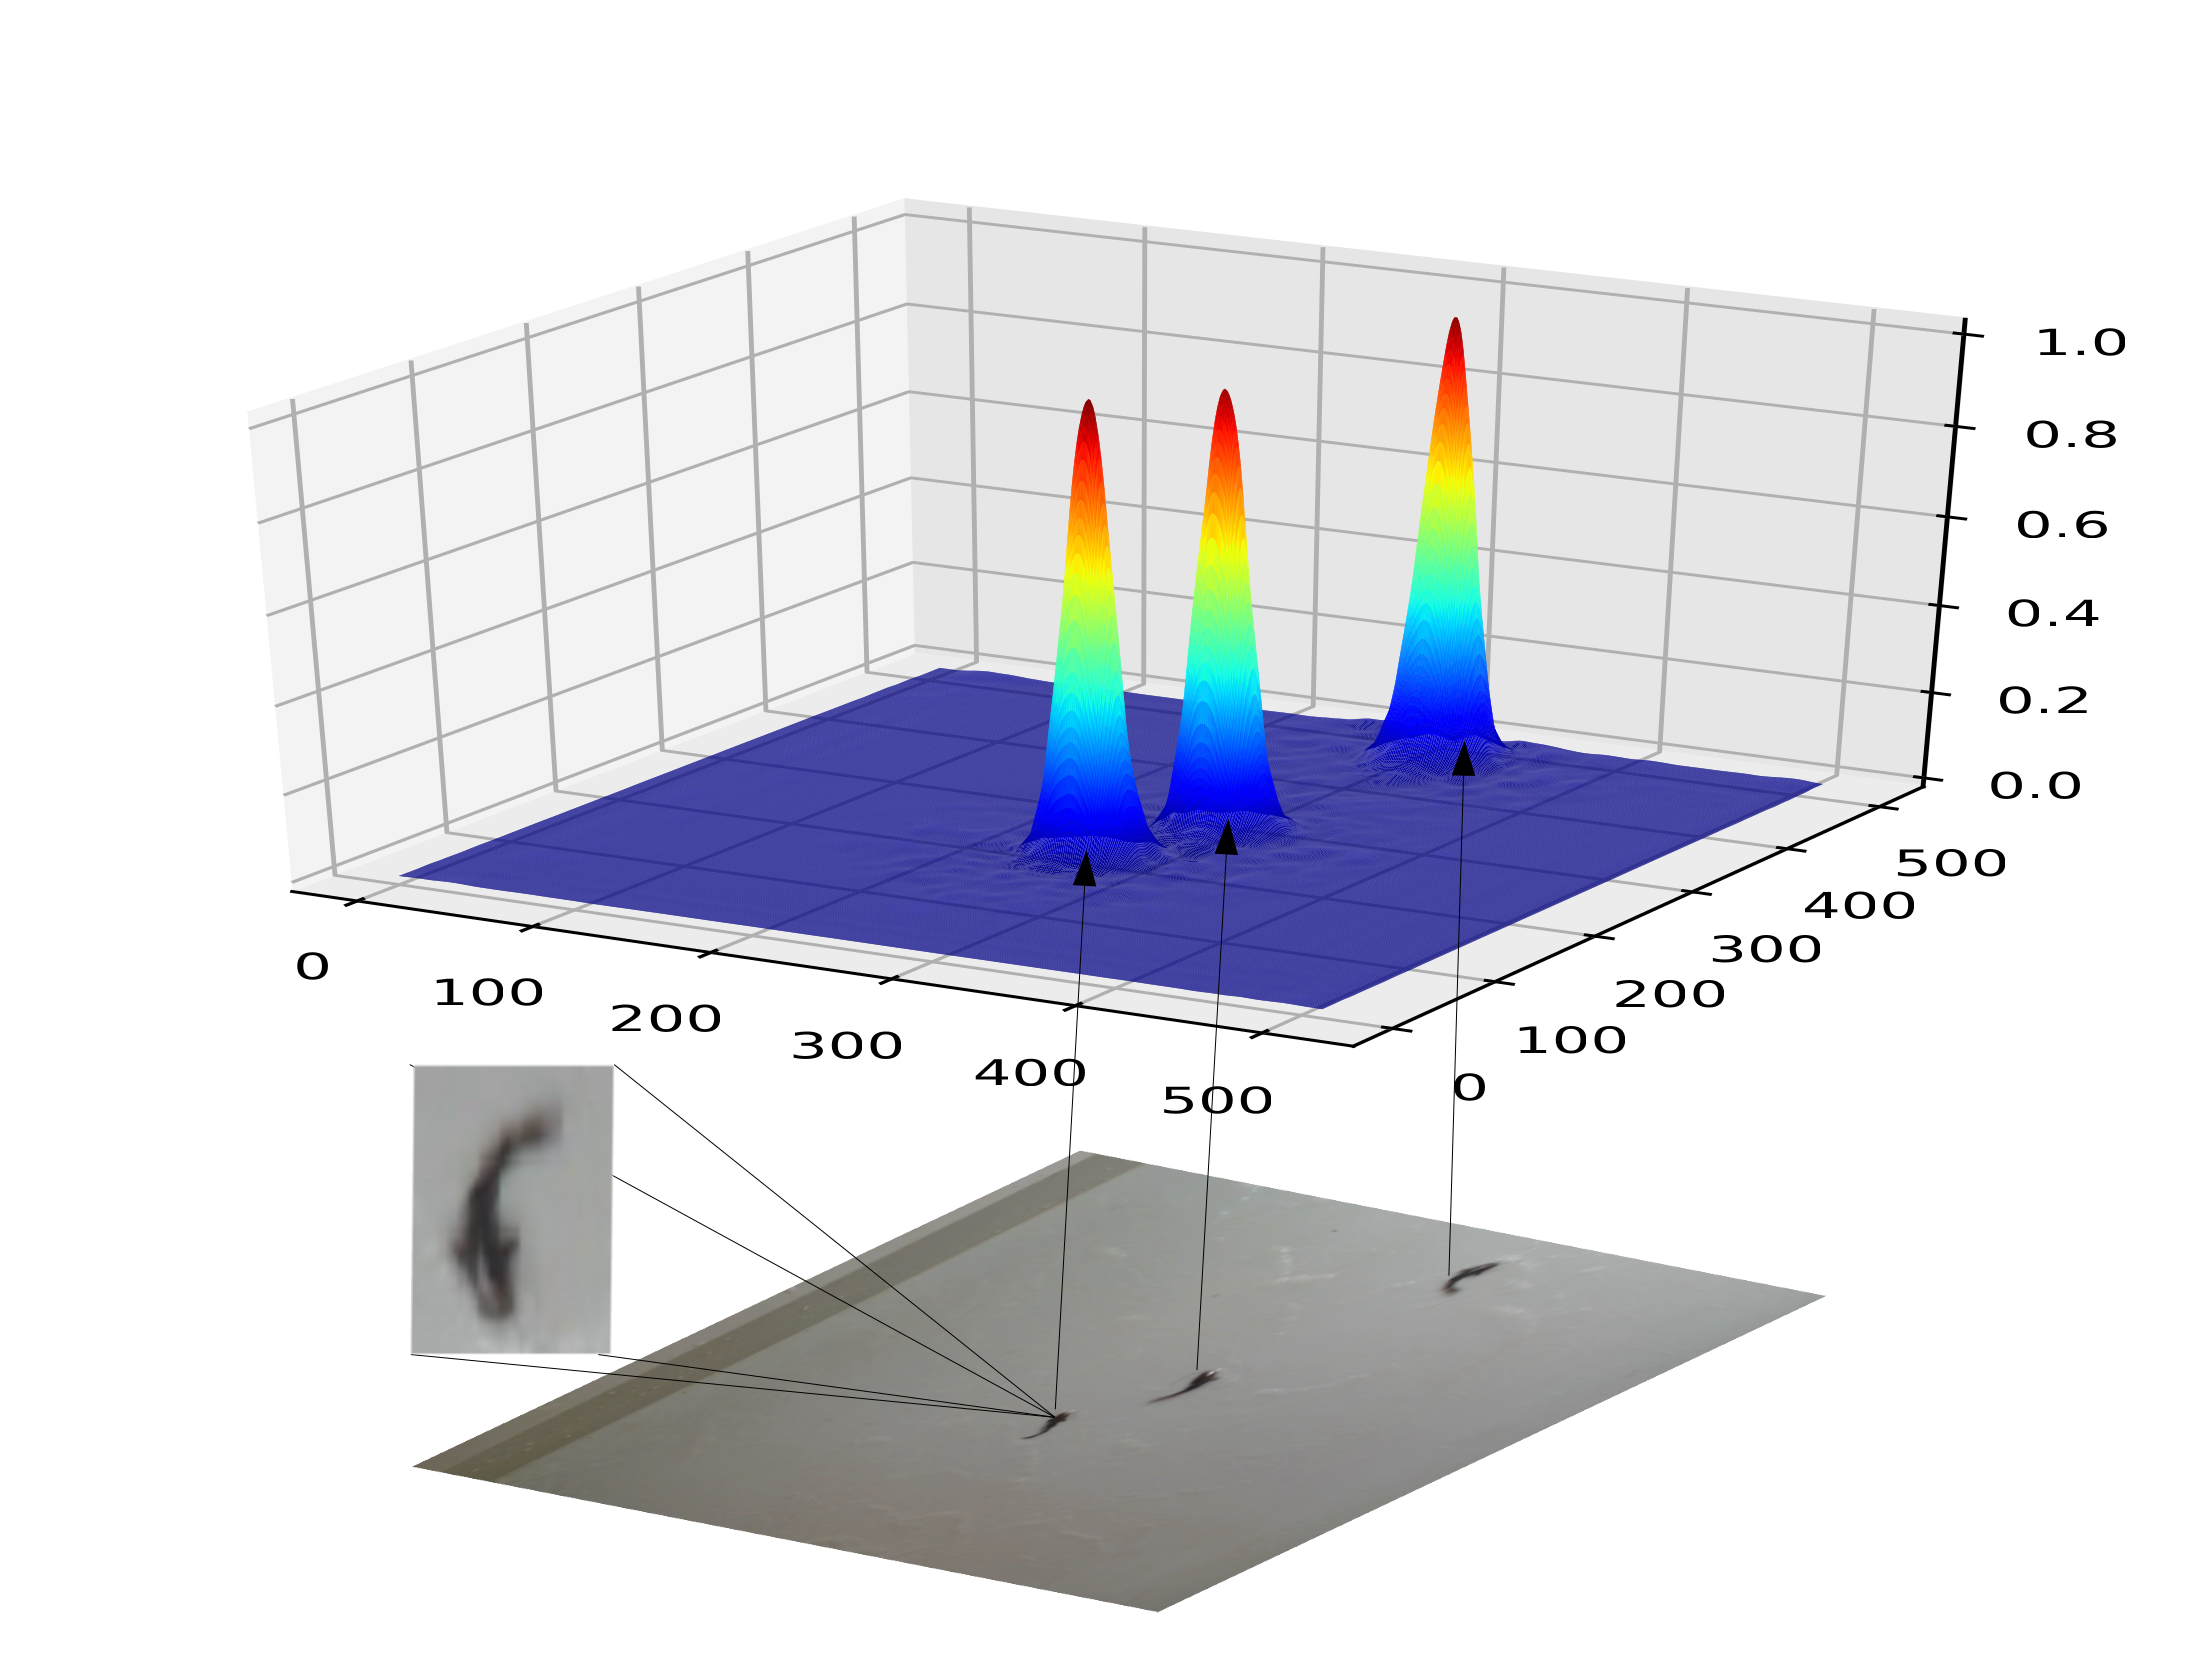
\includegraphics[width=0.9\textwidth]{image/VID06_frame000147.png}}
	\caption{Ilustração do \textit{Heatmap} obtido do \textit{frame} 147 do vídeo número 6, predito pelo modelo treinado por 100 épocas.}
	\label{heatmap}
    \end{figure}

Podemos observar nas imagens da Figura \ref{fig:resultadosQuali} o quadro original, o mapa de densidade, as detecções e a avaliação da métrica \textit{F1} e a estimativa dos vetores de deslocamento.
Todos os peixes presente no quadro foram detectados e os vetores foram estimatidos para as posições anteriores. Neste caso em específico temos dois peixes próximos que foram detectados e contabilizados individualmente.
%Na maioria das vezes os peixes não muito próximos são facilmente detectados.

Haja vista a Seção \ref{subsec:ResultadosQ} os quadros onde a quantidade de alevinos é $\leq 6$, os alevinos são facilmente detectados. Quando a presença de peixes é $\geq 6$ a CNN detecta os alevinos em sua grande maioria, mas existe aqueles que por algum motivo tiveram uma deformação em sua forma na imagem. O movimento realizado pelo peixe diz muito sobre a sua forma.

\begin{figure}[!hbt]
	\centering
	\subfloat[Imagem Original]{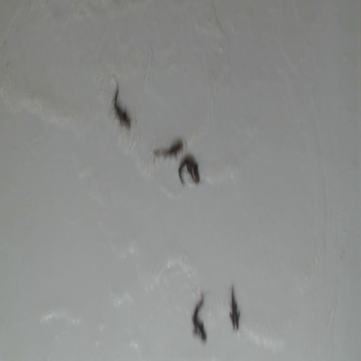
\includegraphics[width=0.4\textwidth]{image/ResultadosQ/VID09_frame000039.png}}\vspace{0.9cm}	
	\subfloat[Mapa de densidade]{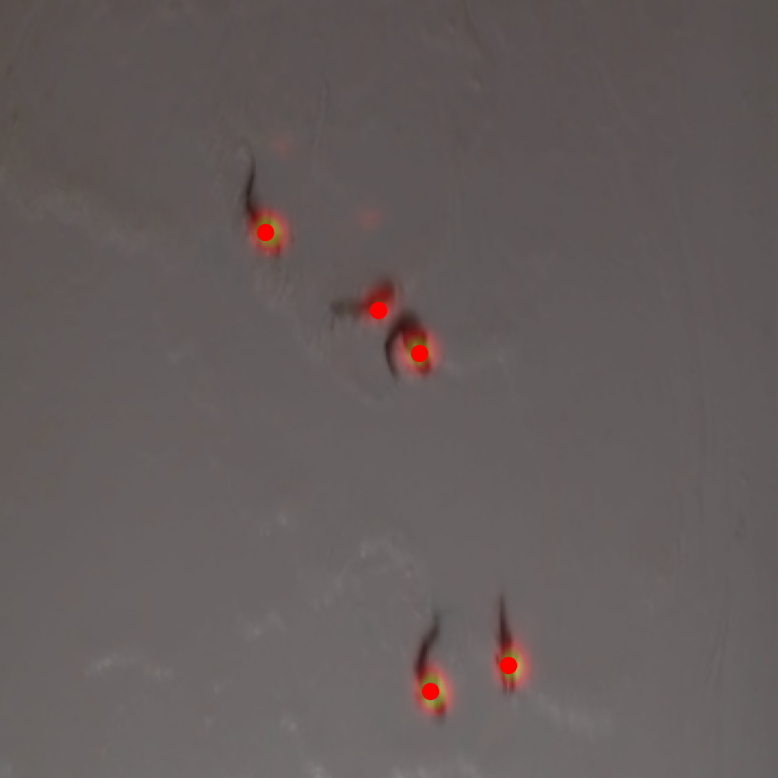
\includegraphics[width=0.4\textwidth]{image/ResultadosQ/VID09_frame000039_points_.png}}\vspace{0.2cm}	
	\subfloat[Predições]{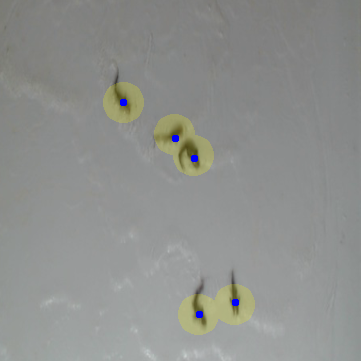
\includegraphics[width=0.4\textwidth]{image/ResultadosQ/VID09_frame000039_points.png}}\vspace{0.2cm}
	\subfloat[Estimativa dos Vetores de Deslocamento]{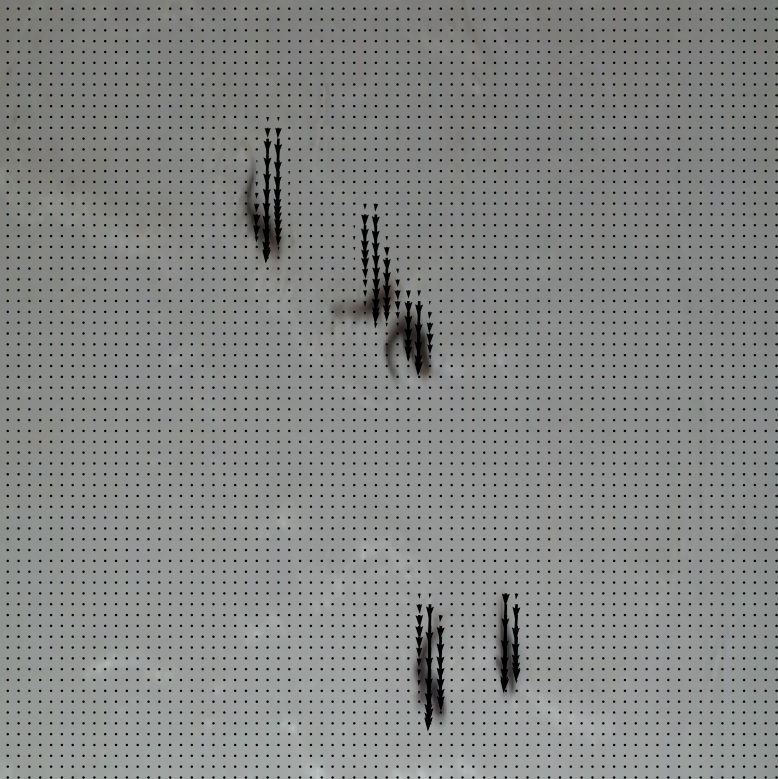
\includegraphics[width=0.4\textwidth]{image/ResultadosQ/VID09_frame000039_vectors.png}}%\vspace{0.2cm}

	\caption{\label{fig:resultadosQuali} Exemplos dos resultados visuais obtidos para o quadro 30 do vídeo 09. A Figura (a) mostra a imagem original, (b) o mapa de densidade, (c) as predições e (d) a estimação dos vetores.
	%As subfiguras (a,b,c) possui as imagens originais, (d,e,f) contém os \textit{heatmaps} obtidos e (g,h,i) os resultados da Métrica F1. 
	%\textbf{TROCAR por IMAGENS da pasta "melhoresResultadosVisuais"}
	}
\end{figure}

Um dos problemas da abordagem proposta esta na detecção correta do alevino quando parte do seu corpo está oclusa na imagem. Isso acontece, pois uma das características da CNN é buscar identificar o alevino considerando uma distribuição de probabilidade de um alevino estar em um pixel. Dessa forma, para que a CNN consiga predizer um alevino, boa parte do formato dele deve aparecer na imagem, para que uma resposta alta a esse padrão seja encontrada. 


Nas imagens presentes na Figura \ref{fig:resultadosJuntos} temos um quadro onde existem três alevinos, porém os dois mais próximos, foram contabilizados apenas como um. Um alevino encontra-se extremamente próximo ao outro, impossibilitando de serem distinguidos a olho nu.
Em alguns quadros na sequência temos que os dois peixes chegam a se separar, porém existem casos em que dois alevinos se movem uniformemente. Essa aproximação confundi a estimativa de vetores, que estima um número de vetores deslocamento diferente.

\begin{figure}[!htb]
	\centering
	\subfloat[Imagem Original]{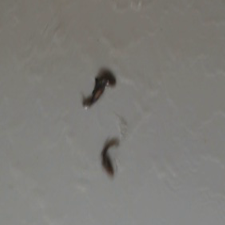
\includegraphics[width=0.35\textwidth]{image/ResultadosQ2/VID11_frame000217.png}}\vspace{0.9cm}	
	\subfloat[\textit{Ground Truth}]{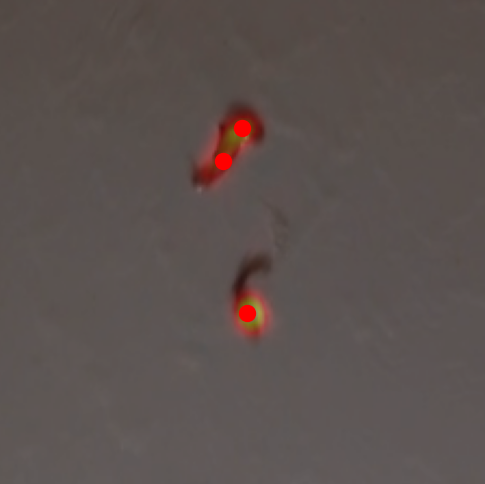
\includegraphics[width=0.35\textwidth]{image/ResultadosQ2/VID11_frame000217_points_gt_.png}}\vspace{0.2cm}	
	\subfloat[Predições]{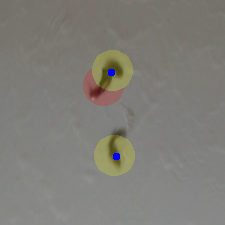
\includegraphics[width=0.35\textwidth]{image/ResultadosQ2/VID11_frame000217_points.png}}\vspace{0.2cm}
	\subfloat[Estimativa dos Vetores de Deslocamento]{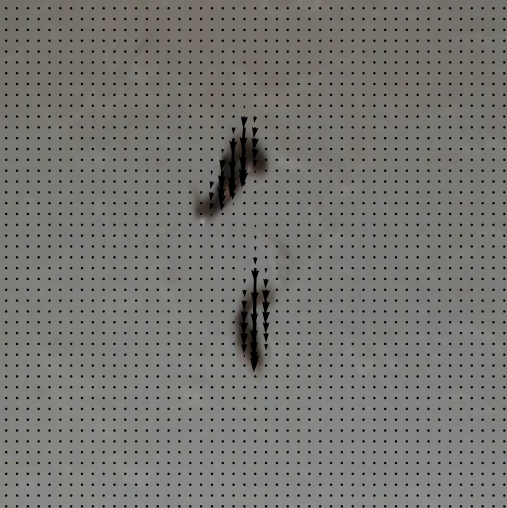
\includegraphics[width=0.35\textwidth]{image/ResultadosQ2/VID11_frame000217_vectors.png}}%\vspace{0.2cm}

	\caption{\label{fig:resultadosJuntos} Exemplos dos resultados visuais obtidos para o quadro 270 do vídeo 11. A Figura (a) nos mostra a imagem original, (b) o mapa de densidade, (c) as predições e (d) a estimação dos vetores.
	%As subfiguras (a,b,c) possui as imagens originais, (d,e,f) contém os \textit{heatmaps} obtidos e (g,h,i) os resultados da Métrica F1. 
	%\textbf{TROCAR por IMAGENS da pasta "melhoresResultadosVisuais"}
	}
	
\end{figure}

%Podemos observar nas imagens \ref{fig:resultadosQuali} que alevinos rigorosamente próximos conseguem ser detectados individualmente. Em especifico na sub figura (a) e (d) temos um exemplos de um frame que contém dois alevinos distantes são identificados corretamente, na sub figura (b) e temos $10$ alevinos presentes nas imagens porém os peixes muito próximos, quase que imperceptível a olho nu, são confundidos pelo método que aponta apenas a presença de $8$ alevinos presentes (figura (e)). A região dos alevinos próximos é apontada como um alevino apenas, isso acontece devido a extrema proximidade que se mantém também nos \textit{frames} anteriores. Nas figuras (c) e (f) nos mostra que os alevinos próximos que mantém uma certa distância, assim como nos quadros anteriores são corretamente detectados pelo método.

%As imagens (b) e (e) da Figura \ref{fig:resultadosQuali} mostra os principais desafios enfrentados pela abordagem proposta. 

Por outro lado, outro grande desafio é detectar corretamente o formato do alevino na imagem. Podemos observar que quase sempre por conta da colisão entre eles os alevinos formam um padrão disforme ao usual.
Apesar desses desafios, o método proposto é capaz de detectar corretamente a grande maioria dos alevinos.
%dois volumes centrais na imagem ao invés de um, podemos ver que a rede pode em alguns casos, predizendo que existem dois alevinos nessas posições. Porém, esse erro tende a diminuir, uma vez que aumentamos o número de imagens de treinamento, pois a rede neural convolucional começa aprender os diferentes formatos que os alevinos podem aparecer nas imagens.

%Nas subfiguras (g,h e i) da Figura \ref{fig:resultadosQuali} temos o resultados obtido pela Métrica F1. Os pontos azuis são as detecções, o círculo amarelo em torno dos peixes são os verdadeiros positivos, ou seja, que foram detectados corretamente. Os círculos vermelhos são os Falsos Negativos, onde há a presença de um peixe porém a arquitetura não o identificou.

%\textbf{DISCUTIR OS RESULTADOS VISUAIS DA NOSSA ABORDAGEM -> na pasta "melhoresResultadosVisuais" tem as imagens onde a técnica detectou corretamente os alevino -> só escolher as 6 melhores e explicar pq ela teve bom resultado..EX: mesmo alevinos grudados, a técnica detectou bem, pois considera o heatmap, etc, etc ...}

%\chapter{Aplicando Análise ROC e Rankings em \cotraining}
%\label{chap:cotraining}


\chapter{Conclusões}
\label{chap:conclusoes}

Neste capítulo são apresentadas as conclusões deste trabalho. Na
Seção~\ref{sec:c:resumo} é realizado um paralelo entre os objetivos desta tese
e os resultados obtidos. Na Seção~ \ref{sec:c:limitacoes} são discutidas
algumas limitações das soluções propostas e na Seção~\ref{sec:c:futuros} são
apresentadas algumas direções de trabalhos futuros.

\section{Resumo dos Objetivos e Principais Resultados}
\label{sec:c:resumo}

O objetivo principal deste trabalho foi apresentar a capacidade de aplicar camadas convolucionais para contar objetos em vídeos, considerando as posições dos mesmos no quadro anterior. Assim são estimados um mapa de densidade e a estimativa de deslocamento de alevino.

O melhor resultado obtido alcançou 98\% de acertos avaliados pela métrica F1, o que nos mostra que a técnica proposta se ajusta positivamente ao conjunto de dados. A métrica de erro MAE afirma que os equívocos cometidos pela rede em camadas é próximos a 0.
O objetivo de refinar o mapa de características utilizando os vetor de deslocamento foi alcançado visto que os melhores resultados se mostraram a partir do processamento das posições que precedem o quadro atual. 

\section{Limitações}
\label{sec:c:limitacoes}

Os alevinos estão em constante movimento nos vídeos, porém existem alguns peixes, geralmente dois(ou até mais) que se juntam e mantém um certo movimento uniforme confundindo a CNN, fazendo-a detectar apenas um peixe naquela posição na imagem. Como o deslocamento dos dois são análogos nos quadros anteriores $I_{t-1}$, no quadro atual $I_{t}$ processado não há possibilidade de se distinguir um do outro. O pico apontado pela CNN para estes peixes extremamente próximos é único e como a detecção é obtida através deles, a CNN detecta estes peixes como um. Na imagem \ref{fig:PeixesPróximos} temos um exemplo de dois peixes que se movimentam igualmente sem indicar uma desaproximação.

\begin{figure}[!ht]
	\centering
	
	\subfloat[quadro 187]{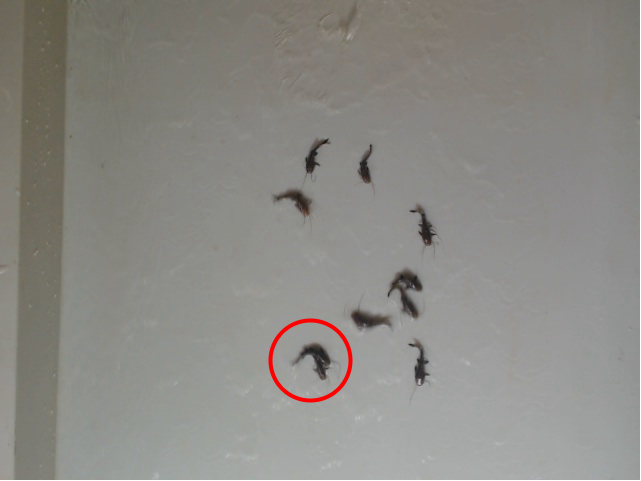
\includegraphics[width=0.46\textwidth]{image/187.png}}\vspace{0.2cm}
	\subfloat[quadro 188]{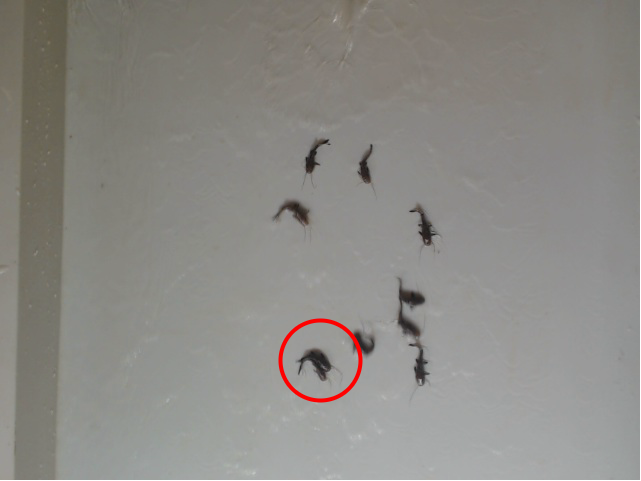
\includegraphics[width=0.46\textwidth]{image/188.png}}\vspace{0.2cm}

	\caption{\label{fig:PeixesPróximos} Exemplos dos peixes extremamente próximos que se movem uniformemente. Imagens do vídeo 06, quadro 187 e 188.
	%\textbf{TROCAR por IMAGENS da pasta "melhoresResultadosVisuais"}
	}
\end{figure}  

\section{Trabalhos Futuros}
\label{sec:c:futuros}

O fato de ocorrer peixes muito próximos nos faz entender que a técnica deverá abordar este tipo de situação. No qual serão testados técnicas para distinguir tais alevinos de maneira com que cada um seja detectado e somado a contagem final.

O método proposto será reavaliado em outro banco de imagens, para averiguar o potencial da técnica em detectar peixes em várias situações do mundo real. Nas imagens da Figura \ref{fig:proxbanco} temos amostras do banco a ser utilizado em novos experimentos.

\begin{figure}[!ht]
	\centering
	
	\subfloat[quadro 4810]{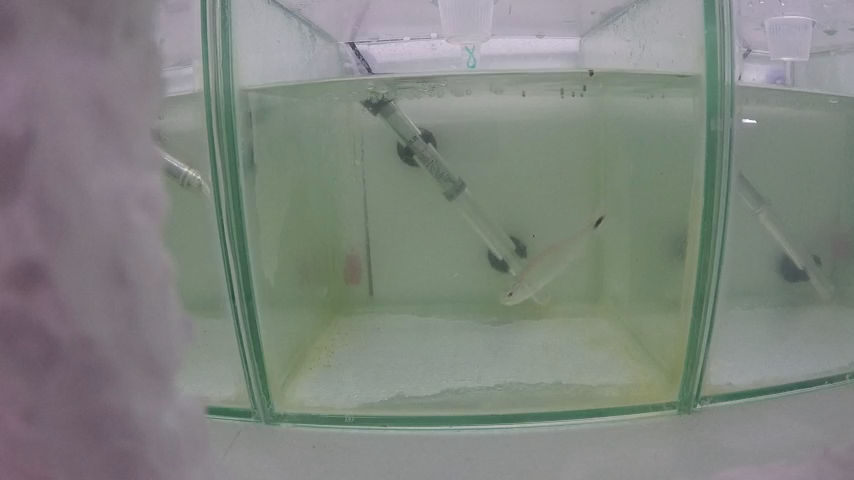
\includegraphics[width=0.8\textwidth]{image/frame0004810.png}}\vspace{0.2cm}
	\subfloat[quadro 6253]{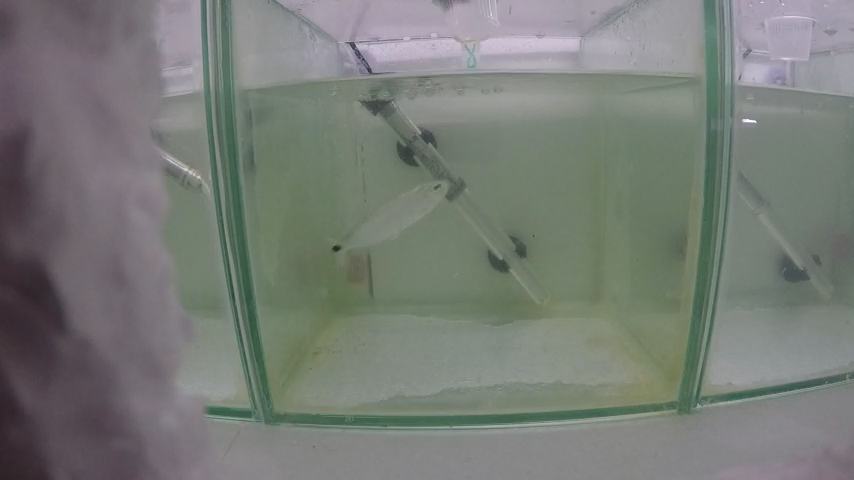
\includegraphics[width=0.8\textwidth]{image/frame0000247.png}}\vspace{0.2cm}

	\caption{\label{fig:proxbanco} Amostra do próximo banco de imagens a ser testado - vídeo 203.
	%\textbf{TROCAR por IMAGENS da pasta "melhoresResultadosVisuais"}
	.}
\end{figure}  




\appendix
\bibliographystyle{apalike}

%%% arquivo .bib
\bibliography{main}
\addcontentsline{toc}{chapter}{Referências}


% Set the ending of a LaTeX document
\end{document}
